%% =====================================================================
%%  Confidence-Guided Adaptive Reconstruction for Windowed QPE
%%  Target venue: MethodsX (Elsevier)
%%  Submission draft. Remaining \PLACEHOLDER markers are author-supplied
%%  fields only (affiliation, ORCID, repo URL, DOI, commit, funding).
%%  Build:  pdflatex main / bibtex main / pdflatex x2
%% =====================================================================
\documentclass[preprint,11pt]{elsarticle}

\usepackage{amsmath,amssymb,amsthm}
\usepackage{booktabs}
\usepackage{graphicx}
\usepackage{xcolor}
\usepackage{array}
\usepackage[hidelinks]{hyperref}
\usepackage{tikz}
\usetikzlibrary{arrows.meta,positioning,fit,backgrounds}
\usepackage[section]{placeins}
\usepackage{algorithm}
\usepackage{algpseudocode}

% ---- float placement: without these, the validation tables drift to the
% ---- end of the document, far from the text that discusses them.
\renewcommand{\topfraction}{0.9}
\renewcommand{\bottomfraction}{0.8}
\renewcommand{\textfraction}{0.07}
\renewcommand{\floatpagefraction}{0.7}
\setcounter{topnumber}{3}
\setcounter{bottomnumber}{2}
\setcounter{totalnumber}{5}

% ---- page efficiency (formatting only; no content is affected) -------
\setlength{\bibsep}{2pt plus 0.3ex}
\setlength{\textfloatsep}{10pt plus 2pt minus 2pt}
\setlength{\intextsep}{10pt plus 2pt minus 2pt}
\setlength{\abovedisplayskip}{6pt plus 2pt minus 2pt}
\setlength{\belowdisplayskip}{6pt plus 2pt minus 2pt}

% ---- draft markers: make every open item greppable and visible -------
\newcommand{\TODO}[1]{\textcolor{red}{\textbf{[TODO: #1]}}}
\newcommand{\PLACE}[1]{\textcolor{blue}{\textbf{[PLACEHOLDER: #1]}}}

% ---- evidentiary labels, carried over verbatim from the source notes -
\newcommand{\PROVEN}{\textsc{(proven)}}
\newcommand{\HEUR}{\textsc{(heuristic)}}
\newcommand{\EMPIR}{\textsc{(empirical)}}
\newcommand{\INVAR}{\textsc{(implementation invariant)}}

\newtheorem{proposition}{Proposition}
\newtheorem{lemma}{Lemma}
\newtheorem{corollary}{Corollary}
\newtheorem{invariant}{Invariant}

% Supplementary Information pointers (SI is a separate document, so these
% are literal rather than \ref, which cannot cross documents).
\newcommand{\SI}{Supplementary Information}
\newcommand{\SIproofs}{\SI{}~Sec.~S1}
\newcommand{\SIaudit}{\SI{}~Sec.~S2}
\newcommand{\SItables}{\SI{}~Sec.~S3}
\newcommand{\SIcalib}{\SI{}~Sec.~S4}
\newcommand{\SIartifacts}{\SI{}~Sec.~S5}

\newcommand{\Cw}{C_w}
\newcommand{\dcov}{\delta_{\mathrm{cov}}}
\newcommand{\Smax}{S_{\max}}
\newcommand{\beammax}{\texttt{beam\_max}}

\journal{MethodsX}

\begin{document}

\begin{frontmatter}

\title{Confidence-Guided Adaptive Reconstruction for Windowed Quantum
Phase Estimation}
% Optional subtitle, if you want one --- uncomment and merge into \title:
% A drop-in classical post-processing replacement for fixed-budget
% candidate reconstruction in modular Shor

\author[inst1]{Sanjay Lakshmanan R}
\ead{rajasanjay21@gmail.com}

\address[inst1]{Department of Computer Science and Engineering,
Amrita Vishwa Vidyapeetham, Chennai, India}

\begin{abstract}
Windowed quantum phase estimation (WQPE) replaces one wide phase register
with several narrow, independently measured windows and reassembles a
full-precision phase classically. The published reconstruction stage
allocates a \emph{fixed} budget to every window --- a constant number of
retained candidates, a constant beam width, and a constant shot count ---
irrespective of how decisive that window's measurement turned out to be.
Characterising our own reproduction of that pipeline, we attributed 72\%
of the failures in the analysed corpus to this uniform allocation rather
than to noise or to any defect in the reconstruction logic.

We describe confidence-guided adaptive reconstruction, a drop-in
customisation of the classical stage that leaves the quantum circuit
unchanged. A per-window posterior comparison statistic $\Cw$, computed
from counts already measured, quantifies how decisively the most-observed
bit pattern leads the runner-up, and drives three independently
switchable modules: coverage-based candidate retention (B),
ambiguity-scaled beam width (C), and confidence-gated shot stopping (D).
B and D carry the stronger independent evidence; C is evaluated chiefly
as a component of the full framework. With all three disabled the
implementation reduces to the published pipeline, verified trial by
trial.

On a 144-cell grid starving all three budgets simultaneously, the
published pipeline fails 47.9\% of the time; enabling all three modules
raises end-to-end factorisation success from 52.1\% to 100\%, and across
three pre-specified held-out instances the combination reaches
97.9--100\%. Matched-resource controls qualify this and are reported as a
primary finding: given each module's own realised budget spread uniformly
and without confidence guidance, no individual module is distinguishable
from its control. The evidence therefore supports \emph{automatic,
instance-adaptive selection of the reconstruction budget} --- removing the
need to choose it correctly in advance --- rather than a demonstrated
superiority of confidence-guided placement over an equivalent uniform
allocation.

Validation is noiseless, simulation-only, and confined to
$N\in\{15,21\}$ at orders $r\in\{2,4,6\}$, a ceiling imposed by a
measured compilation cliff rather than chosen; and $\Cw$, while an
effective ranking signal, is measurably overconfident (Brier 0.2239) and
must not be read as a calibrated probability.
\end{abstract}

\begin{keyword}
Quantum phase estimation \sep Shor's algorithm \sep classical
post-processing \sep adaptive resource allocation \sep Bayesian posterior
comparison \sep beam search
\end{keyword}

\end{frontmatter}

% =====================================================================
\section*{Highlights}
\begin{itemize}\itemsep2pt
\item In the analysed failure corpus, 72\% of observed failures were
      attributed to classical reconstruction-budget starvation.
\item A per-window Bayesian statistic sets candidate, beam and shot
      budgets from the already-measured counts.
\item Reconstruction success is 97.9--100\% across four instances; the
      quantum circuit is unchanged.
\item Matched-resource controls attribute the gain to automatic budget
      selection, not to placement.
\end{itemize}

% =====================================================================
\section*{Specifications table}

\begin{center}
\small
\begin{tabular}{@{}p{0.30\linewidth}p{0.64\linewidth}@{}}
\toprule
\textbf{Subject area} & Physics and Astronomy \\
\midrule
\textbf{More specific subject area} & Quantum computing; quantum
algorithms; classical post-processing for quantum phase estimation \\
\midrule
\textbf{Name of your method} & Confidence-Guided Adaptive Reconstruction
for Windowed Quantum Phase Estimation \\
\midrule
\textbf{Name and reference of original method} & Windowed quantum phase
estimation with carry-aware candidate stitching, as specified by Shukla
and Vedula \cite{wqpe2025,modularshor2025} (Algorithm 3 of the latter). \\
\midrule
\textbf{Resource availability} & Code, experiment scripts and all raw
result data: \url{https://github.com/Shadow-46/QuantumPhaseReconstruction} (Apache-2.0). An
archived snapshot will be deposited in a persistent repository and its
DOI supplied at acceptance. Dependencies: Python 3.12,
Qiskit \cite{qiskit2024} $\geq$ 2.5, Aer $\geq$ 0.15, SciPy $\geq$ 1.14,
NumPy $\geq$ 2.0, scikit-learn $\geq$ 1.4. No quantum hardware required.
Script-to-artifact map: \SIartifacts{}. \\
\bottomrule
\end{tabular}
\end{center}

\noindent
\textit{Note on scope.} This article customises only the \emph{classical
reconstruction} stage of the original method. No change is made to the
quantum circuit, its qubit count, its depth, or its sampling procedure.
The method is therefore reusable by any implementation of windowed phase
estimation that produces per-window measurement counts, independently of
how those counts were generated.

% =====================================================================
\section*{Graphical abstract}

\noindent
A landscape rendering of Figure~\ref{fig:schematic}, with the three
adaptive modules annotated by the fixed quantity each replaces
($k\to m_w$, $P\to P'$, $S_w\to$ resampled $S_w$), and a caption strip
carrying the canonical comparison: published fixed-budget reconstruction
$52.1\%$, matched-resource control $73.6\%$, adaptive pipeline $100\%$.
Supplied as a separate image file at submission.

% =====================================================================
\section*{Introduction}
\label{sec:intro}

Shor's algorithm \cite{shor1997} reduces integer factorisation to
order-finding, and order-finding to quantum phase estimation
\cite{kitaev1995,cleve1998,nielsenchuang}. Textbook QPE requires a phase
register as wide as the requested precision, which is exactly the
resource near-term hardware does not have. The windowed formulation
\cite{wqpe2025,modularshor2025} removes that requirement by partitioning
the phase register into narrow, independently measured, overlapping
windows and reassembling the full-precision phase classically. The
quantum saving is real, and it is bought with classical work: the
reconstruction stage must now recover one phase from $W$ partial,
individually ambiguous measurements.

That classical stage is where this article intervenes. Three of its
quantities are compile-time constants in the published method --- how
many candidate bit patterns to retain per window, how wide a beam to
carry through stitching, and how many shots to spend per window --- and
they are identical for every window of every instance, regardless of how
decisive that window's measurement turned out to be. Our black-box
characterisation of a from-scratch reproduction found that this uniform
allocation, not noise and not any defect in the reconstruction logic, is
the dominant failure mechanism we were able to observe: of the 94
failures the campaign produced, 72\% were attributed to classical budget
starvation, and a grid starving all three budgets at once fails 47.9\% of
the time on an instance the same pipeline solves trivially when any one
budget is relaxed. Both figures characterise the corpus we analysed, not
windowed phase estimation in general.

The customisation we describe replaces each of the three constants with a
quantity computed from the counts that have already been measured, via a
per-window posterior comparison statistic. It changes no circuit, adds no
qubit, and reduces exactly to the published pipeline when switched off ---
a property of the implementation that we verified trial by trial rather
than assumed.

One scoping note shapes how the rest of this article is written.
Enabling all three modules removes essentially every failure in the
regime where failures occur, but a module compared against a control
handed its \emph{own} realised budget to spend uniformly is
statistically indistinguishable from that control. The defensible
contribution is therefore automatic budget selection, not superior
placement of a given budget; Sec.~\ref{sec:discussion} develops this.

\paragraph{Summary of contributions.} Each item names where it is
established.

\begin{enumerate}\itemsep2pt
\item \textbf{A per-window posterior comparison statistic $\Cw$} for
windowed phase reconstruction, defined as an exact two-proportion
Bayesian comparison over the top-two observed patterns
(Sec.~\ref{sec:cw}), with proven ordinal properties
(Table~\ref{tab:properties}; derivations in \SIproofs{}).

\item \textbf{Three independently switchable reconstruction modules}
driven by the sampled counts --- coverage-based candidate retention (B),
ambiguity-scaled beam width (C), and confidence-gated shot stopping (D)
(Secs.~\ref{sec:moduleB}--\ref{sec:moduleD},
Algorithm~\ref{alg:adaptive}) --- with a \textbf{verified equivalence to
the published baseline} when all three are disabled
(Invariant~\ref{prop:baseline}), which is what makes the method safe to
adopt incrementally. The three are \emph{not} equally supported by the
evidence: B and D each carry a large independent effect, whereas C's
isolated contribution is small and does not survive multiple-comparison
correction, so we evaluate it chiefly as part of the full framework
(Secs.~\ref{sec:heldout}, \ref{sec:matched}).

\item \textbf{A reusable adoption protocol} (Sec.~\ref{sec:protocol}) and
a cost analysis (Sec.~\ref{sec:cost}) separating classical asymptotics,
whose complexity class is unchanged under the bounded caps analysed here,
from module D's additional \emph{quantum} sampling, which is bounded but
real.

\item \textbf{Seed-paired validation on four instances} --- the canonical
grid plus three pre-specified held-out instances, 144 trials each
(Secs.~\ref{sec:results}--\ref{sec:heldout}) --- and
\textbf{matched-resource controls} isolating adaptivity from budget size
(Sec.~\ref{sec:matched}). The controls are the paper's most consequential
result and are partly negative: no single module beats a control given
the same realised budget uniformly, while the combination does.

\item \textbf{A calibration study of $\Cw$} (Sec.~\ref{sec:calibration})
establishing that it carries useful ranking information but is not a
calibrated probability estimate, and
a matter-of-fact account of a self-caught audit-script error that
reversed one of our own earlier headline findings
(Sec.~\ref{sec:retraction}).
\end{enumerate}

% =====================================================================
\section{Method details}

\subsection{The original method and the three constants it fixes}
\label{sec:baseline}

Quantum phase estimation recovers an eigenphase $\varphi$ of a unitary
$U$ from measurements of a phase register \cite{kitaev1995,cleve1998}.
In Shor's order-finding reduction \cite{shor1997}, $U_a\lvert
y\rangle=\lvert ay \bmod N\rangle$ has eigenphases $s/r$ for the
multiplicative order $r=\mathrm{ord}_N(a)$; continued-fraction expansion
of a measured phase recovers $r$, and factors follow from
$\gcd(a^{r/2}\pm1,N)$ \cite{nielsenchuang}.

Standard QPE requires a phase register as wide as the requested
precision, which is prohibitive on shallow hardware. The windowed
formulation \cite{wqpe2025,modularshor2025} instead partitions the
$\ell$-bit phase interval into $W$ overlapping windows. Window $w$
covers bit positions $[\mathrm{start}_w,\mathrm{start}_w+\mathrm{width}_w)$
with $\mathrm{start}_{w+1}=\mathrm{start}_w+\mathrm{width}_w-o$ for
overlap $o$, and is measured by its own circuit allocating only
$\mathrm{width}_w$ phase qubits --- never $\ell$. Circuit width is thus
decoupled from total precision, which is the formulation's central
resource claim.

The cost of that decoupling is borne entirely by the classical stage,
which must reassemble one full-precision phase from $W$ partial and
possibly ambiguous local measurements. Given per-window count
dictionaries $\mathrm{counts}_w:\{0,1\}^{\mathrm{width}_w}\to
\mathbb{Z}_{\geq0}$ with $S_w=\sum_b \mathrm{counts}_w(b)$ shots, the
published pipeline proceeds in three steps:

\begin{enumerate}\itemsep1pt
\item \textbf{Candidate generation.} Rank each window's observed patterns
by empirical probability $\hat p_w(b)=\mathrm{counts}_w(b)/S_w$ and
retain the top $k$ (\texttt{candidate\_count}), each encoded at its
absolute bit position.
\item \textbf{Carry-aware beam stitching.} Extend paths across adjacent
windows, admitting a pair when its overlapping bits agree exactly or
after one legitimate single-bit borrow; score paths by the product of
candidate probabilities and retain the top $P$ (\texttt{max\_paths}) at
each level.
\item \textbf{Order recovery.} Apply continued-fraction expansion to each
stitched phase in ranked order until one yields a non-trivial
factorisation.
\end{enumerate}

Three quantities are fixed constants here, chosen at configuration time
and identical for every window of every instance: the candidate count
$k$, the beam width $P$, and the per-window shot count $S_w$. Our method
replaces all three with data-dependent quantities computed from the
already-sampled counts, as shown schematically in
Figure~\ref{fig:schematic}. A symbol table is given in \SIproofs{};
every symbol is also defined where it first appears below.

\begin{figure}[htbp]
\centering
\resizebox{\linewidth}{!}{%
\begin{tikzpicture}[
  font=\small,
  box/.style={draw, rounded corners, align=center, minimum height=1.05cm, minimum width=2.05cm, inner sep=3pt},
  mod/.style={draw, dashed, rounded corners, align=center, minimum height=0.85cm, fill=gray!8, inner sep=3pt},
  arr/.style={-{Latex[length=2.2mm]}, thick},
  node distance=6mm
]

\node[box] (sample) {Windowed\\quantum sampling\\[1pt]\footnotesize $W$ shallow\\circuits, widths\\$\mathrm{width}_1,\dots,\mathrm{width}_W$};
\node[box, right=of sample] (counts) {Per-window\\counts $\mathrm{counts}_w$\\[1pt]\footnotesize $S_w$ shots each};
\node[box, right=of counts] (candgen) {Candidate\\generation};
\node[box, right=of candgen] (stitch) {Carry-aware\\beam stitching};
\node[box, right=of stitch] (order) {Continued-fraction\\order recovery};
\node[box, right=of order] (factors) {Factors of $N$};

\draw[arr] (sample) -- (counts);
\draw[arr] (counts) -- (candgen);
\draw[arr] (candgen) -- (stitch);
\draw[arr] (stitch) -- (order);
\draw[arr] (order) -- (factors);

\node[mod, below=9mm of counts] (moduleD) {Module D: $\Cw$ per window;\\below threshold $\Rightarrow$ more shots\\(cap $\Smax$)};
\node[mod, below=9mm of candgen] (moduleB) {Module B: retain\\candidates to coverage\\$\dcov$ (adaptive $m_w$)};
\node[mod, below=9mm of stitch] (moduleC) {Module C: beam width\\$P'$ scales with\\coverage-expansion rate\\(cap $\beammax$)};

\draw[arr] (moduleD) -- (counts);
\draw[arr, dashed] (moduleD.north) -- ++(0,3mm) -| (sample.south);
\draw[arr] (moduleB) -- (candgen);
\draw[arr] (moduleC) -- (stitch);

\end{tikzpicture}%
}
\caption{Method schematic. The published pipeline (top row, solid) samples
each window once at a fixed shot budget, retains a fixed candidate count,
and stitches with a fixed beam width. The three adaptive modules
(dashed, bottom) replace each fixed budget with a quantity computed from
the already-sampled counts: module D re-samples ambiguous windows before
candidate generation proceeds (dashed feedback arrow into the sampling
stage), module B expands candidate retention to a target probability
mass, and module C widens the beam in proportion to how often module B
needed to expand coverage. All three modules are independently
switchable and the pipeline reduces to the published baseline when all
three are disabled.}
\label{fig:schematic}
\end{figure}



\subsection{Motivating evidence: fixed budgets are the binding constraint}
\label{sec:motivation}

The method was not designed from intuition. It was designed against a
prior black-box failure-mode characterisation of our own reproduction of
the published pipeline, which we summarise here only insofar as it
motivates the design; the full campaign is reported separately.

Varying any single parameter in isolation produces no failures at all:
across 435 one-factor-at-a-time trials --- sweeping total precision
(4--12), window size (2--8), overlap (0--3), candidate count (1--16),
beam width (1--4096) and shots (16--16384) on three small $(N,a)$ pairs
--- every trial succeeded. This is a genuine null result with a specific
cause: at the small multiplicative orders reachable in our environment
the continued-fraction multiplier search is extremely forgiving, so
theoretically under-resolved configurations still recover the correct
order.

Starving several budgets \emph{together} tells the opposite story. On the
same instance ($N=21$, $a=19$, $r=6$), a 144-cell grid simultaneously
constraining $k\in\{1,2\}$, $P\in\{1,2\}$ and $S_w\in\{4,8,16\}$ while
maximising precision ($\ell\in\{16,24,32\}$) and overlap ($o\in\{0,3\}$)
failed on 69 of 144 trials --- 47.9\%, with zero injected noise and zero
corruption. Replaying every failure observed anywhere in the campaign
through a fixed counterfactual ladder (exact bits $\to$ widened beam
$\to$ exhaustive candidates $\to$ noise disabled $\to$ ten-fold shots)
attributed 68 of 94 failures (72\%) to classical budget starvation rather
than to noise, corruption, or any defect in the reconstruction logic. Of
those, 48 were resolved by additional shots alone; 20 resisted every
single-axis relaxation and needed candidate budget \emph{and} beam width
relaxed jointly.

That attribution defines the design target precisely. The failures are
not caused by the carry-aware overlap check, by the windowing geometry,
or by the quantum sampling; they are caused by spending a fixed classical
budget on windows that needed an unequal one. Figure~\ref{fig:pareto}
shows the resulting failure-mode distribution.

\begin{figure}[htbp]
\centering
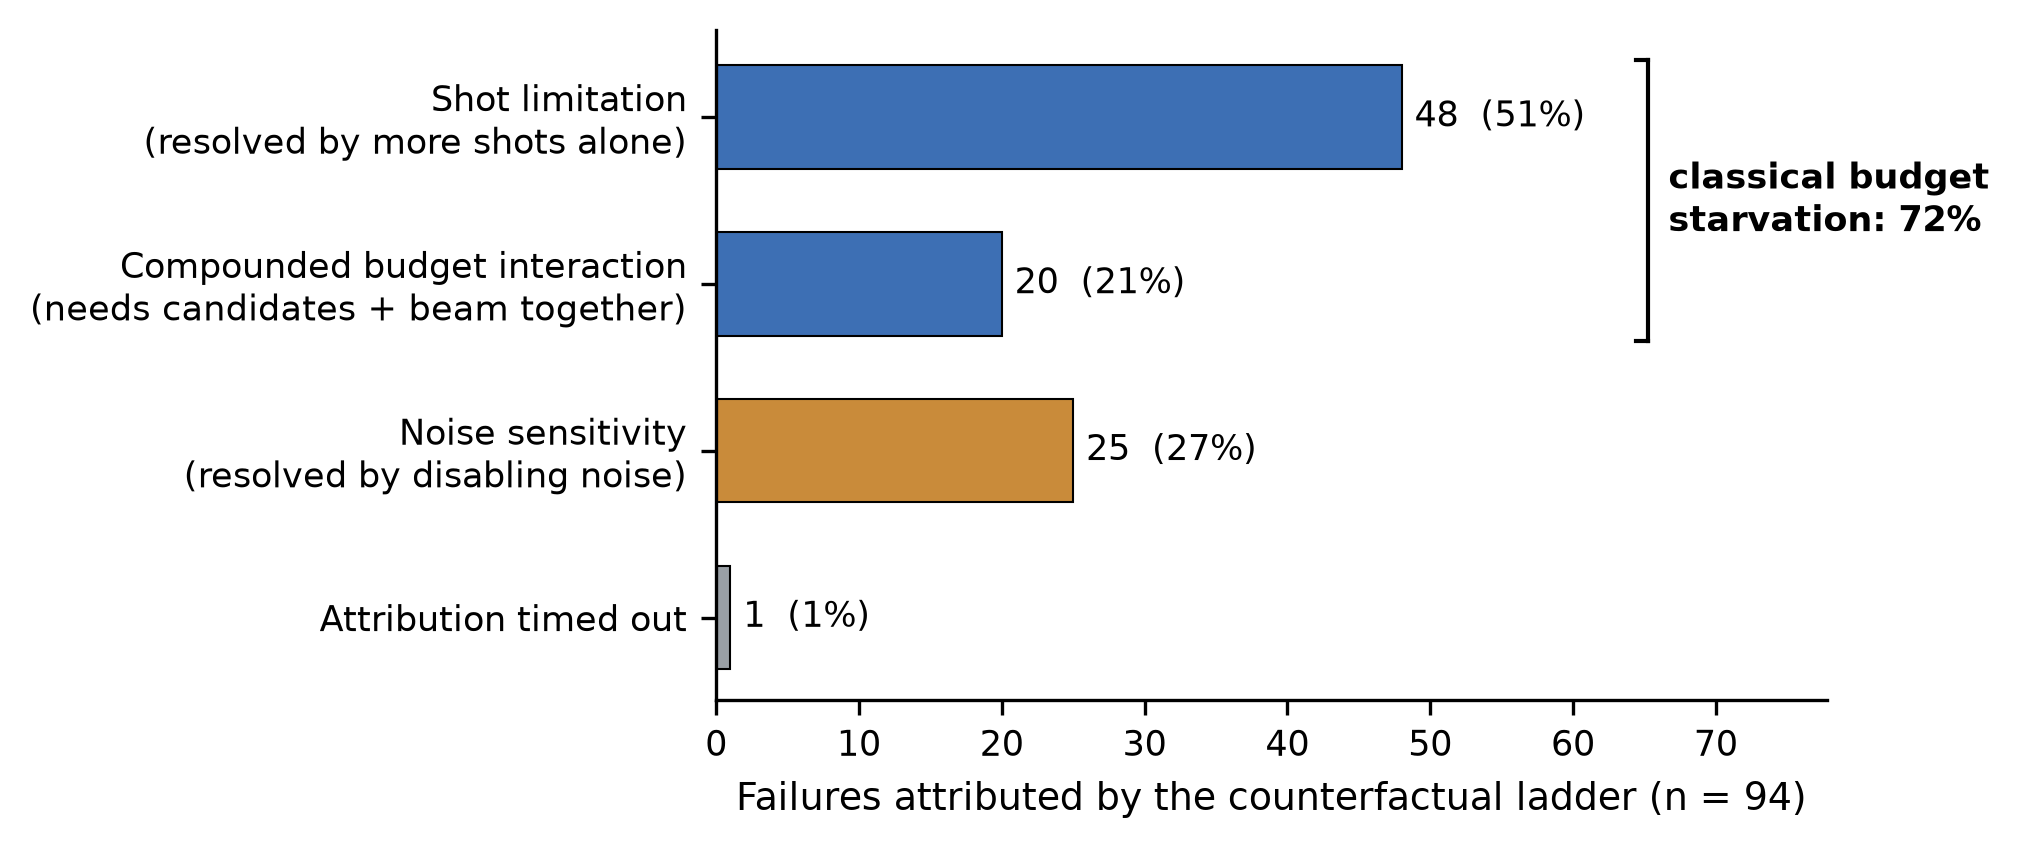
\includegraphics[width=\linewidth]{../Data/failure_study/plots/paper_fig2_failure_attribution.png}
\caption{\textbf{Which mechanism should a fix target?} Root-cause
attribution of all 94 failures observed anywhere in the characterisation
campaign, each replayed through the same counterfactual ladder and
assigned to the first rung that recovers it. Within this corpus the two
classical-budget mechanisms (blue) account for 72\% of failures between
them: 48 that
additional shots alone resolve, and 20 that resist every single-axis
relaxation and need candidate budget and beam width widened together.
Noise (orange) accounts for 27\%. This distribution is what selects the
classical reconstruction stage, rather than the circuit or the noise
model, as the place to intervene. Rendered from
\texttt{phase5\_attribution.csv}.}
\label{fig:pareto}
\end{figure}

\subsection{Relation to existing adaptive and Bayesian approaches}
\label{sec:related}

Adaptivity and Bayesian inference are both well established in quantum
estimation, so it is worth being precise about what is and is not new
here.

\emph{Bayesian amplitude- and phase-estimation methods}
\cite{bae2025,biqae2026,vqae2022} maintain a posterior over the estimated
quantity and use it to choose the next \emph{quantum} query --- which
circuit to run, at what depth, for how many shots --- to reduce quantum
query complexity. Module D is a deliberately narrower relative of that
idea. The difference is what the posterior governs: those methods
optimise the quantum sampling schedule, whereas modules B and C spend no
quantum resources at all and reallocate a purely classical budget over
counts already measured. The two are complementary, and nothing prevents
combining them.

\emph{Existing windowed-reconstruction pipelines}
\cite{wqpe2025,modularshor2025} already contain multi-candidate
retention, carry-aware stitching and beam-search pruning; we reproduce
all three unchanged. What they lack is any rule connecting the budget a
window receives to how ambiguous that window's measurement was: overlap
is static, and the candidate count and beam width are constants.

\emph{Exhaustive reconstruction} --- searching every consistent path
rather than a bounded beam --- is the exactness endpoint of the same axis,
at a cost combinatorial in the number of windows. Our framework
approaches it in the joint limit $\Smax\to\infty$, $\dcov\to0$,
$\beammax\to\infty$, so the relationship is one of degree rather than
kind. We make no claim about specific published exhaustive or
dynamic-programming algorithms, having surveyed the class rather than
benchmarked a named implementation.

Table~\ref{tab:novelty} places the present work against these lines
along the dimensions that distinguish them. The reproduced components
occupy the same cells as the source method by construction; the two
rightmost columns are where this article differs, and the adaptive-sampling
cell differs only in the restricted sense its footnote records.

\begin{table}[htbp]
\centering\footnotesize
\caption{Positioning against the cited prior work.
\checkmark~= present and adaptive; \emph{fixed} = present but set at
configuration time; ---~= not applicable to that method. Reproduced
components ($\ast$) occupy the same cells as the source method by
construction; the two rightmost columns are where this article differs. The
table compares only works cited here, and only on dimensions those works
address; it is not a survey.}
\label{tab:novelty}
\setlength{\tabcolsep}{3.2pt}
\begin{tabular}{@{}p{0.215\linewidth}cccccc@{}}
\toprule
 & \shortstack{Windowed\\circuits}
 & \shortstack{Multi-\\candidate}
 & \shortstack{Carry-aware\\stitching}
 & \shortstack{Bounded\\beam}
 & \shortstack{Adaptive\\sampling}
 & \shortstack{\textbf{Adaptive}\\\textbf{cl. budget}} \\
\midrule
Standard QPE \cite{kitaev1995,cleve1998}
  & ---        & ---            & ---        & ---            & ---        & --- \\[2pt]
Windowed / modular WQPE \cite{wqpe2025,modularshor2025}
  & \checkmark & \emph{fixed}   & \checkmark & \emph{fixed}   & ---        & --- \\[2pt]
Bayesian amplitude / phase estimation \cite{bae2025,biqae2026,vqae2022}
  & ---        & ---            & ---        & ---            & \checkmark & --- \\[2pt]
\textbf{This work}
  & \checkmark$^{\ast}$ & \checkmark & \checkmark$^{\ast}$ & \checkmark
  & \checkmark$^{\dagger}$ & \checkmark \\
\bottomrule
\end{tabular}

\vspace{3pt}
\begin{minipage}{\linewidth}\footnotesize
$\ast$~Reproduced unchanged from the source method, not a contribution of
this article. \quad
$\dagger$~Module D adapts only \emph{how many shots} an already-specified
window circuit receives; it never changes which circuit is run, unlike
the Bayesian methods in row 3.
\end{minipage}
\end{table}

The gap we address is therefore specific: \emph{a rule that sets the
classical reconstruction budget --- candidates retained, beam width, and
shots per window --- from the measured counts, leaving the quantum
circuit and its resource profile untouched}. We have not found this
combination proposed for windowed phase estimation, and our survey
covered Bayesian, maximum-likelihood, machine-learning,
dynamic-programming, beam-search and graph-search reconstruction. We
state that as the outcome of a survey rather than as an absence proof.

Two qualifications belong here rather than in a later section: the
statistic is confidence-\emph{driven}, not confidence-\emph{calibrated}
(Sec.~\ref{sec:calibration}), and what it contributes at the scales we
can reach is the automatic selection of a budget, not a superior
placement of one (Sec.~\ref{sec:matched}). A reader comparing against a
well-tuned fixed budget should expect parity; the value on offer is that
no tuning is needed to reach it.

\subsection{The posterior comparison statistic $\Cw$}
\label{sec:cw}

The one new piece of mathematics the framework depends on is a per-window
statistic that is aware of how much evidence a window's ranking actually
rests on. Let $b^{(1)}_w$ and $b^{(2)}_w$ be the two most-observed bit
patterns in window $w$, with counts $n_1 \ge n_2$ out of $S_w$ shots.
Model each pattern's marginal success count as Binomial and place an
independent Jeffreys prior $\mathrm{Beta}(\tfrac12,\tfrac12)$
\cite{jeffreys1946} on each marginal probability, giving posteriors
$X_i\sim\mathrm{Beta}(\alpha_0+n_i,\ \alpha_0+S_w-n_i)$, $i\in\{1,2\}$,
$\alpha_0=\tfrac12$. Define

\begin{equation}
\Cw \;\mathrel{:=}\; \Pr\!\big[X_1 > X_2\big]
\;=\; \int_0^1 f_{X_1}(x)\,F_{X_2}(x)\,\mathrm{d}x ,
\label{eq:cw}
\end{equation}

with $f_{X_1}$ the density of $X_1$ and $F_{X_2}$ the distribution
function of $X_2$. Equation~\eqref{eq:cw} is evaluated directly, so
$\Cw$ is exactly the stated posterior quantity up to quadrature
tolerance.

\paragraph{What $\Cw$ is, stated precisely.} Under the sampling model
(A1) \emph{and} the working independence assumption (A2) of
Sec.~\ref{sec:assumptions}, $\Cw$ is the posterior probability that
$p_w(b^{(1)}_w) > p_w(b^{(2)}_w)$. Assumption (A2) is false --- the two
counts are negatively correlated coordinates of one $K_w$-way multinomial,
so the exact posterior is a Dirichlet marginal comparison, not a
comparison of two independent Beta variables --- and the size of the
resulting error is measured in Sec.~\ref{sec:calibration}. We therefore
use the term \textbf{posterior comparison statistic} throughout, and we
do \emph{not} describe $\Cw$ as a calibrated probability, a confidence
level with guaranteed coverage, or an error rate. Its established
properties are ordinal (Table~\ref{tab:properties}); its role in the
method is to \emph{rank}
windows by how thin their evidence is, and every use downstream depends
only on that ranking together with one threshold whose value is a tuning
parameter rather than a guarantee.

\paragraph{Why this statistic and not a simpler one.}
Raw probability, top-1/top-2 margin, and entropy over the observed counts
are all \emph{sample-size-blind}. A $2/4$ split and a $500/1000$ split
score identically under every one of them, even though the first is
nearly uninformative and the second nearly certain. Since the dominant
measured failure mode is under-sampling rather than genuine ambiguity
(Sec.~\ref{sec:motivation}), a statistic that cannot tell these apart is
the wrong instrument. Equation~\eqref{eq:cw} is the minimal quantity that
separates them from a single closed definition. A likelihood-ratio test
between ``$b^{(1)}$ true'' and ``$b^{(2)}$ true'' behaves almost
identically --- both reduce to a function of the margin over its standard
error --- so nothing is gained by preferring it, and the posterior form
states more transparently what is being computed. We claim only that
$\Cw$ separates the two regimes with a single unconditional formula, not
that it is optimal among statistics that could do so.

\paragraph{Numerical evaluation.} For general real shape parameters,
$\Pr[X_1>X_2]$ between independent Beta variables has no elementary
closed form. A finite closed-form sum exists when one shape parameter is
a positive \emph{integer}, but here $b_i=0.5+(S_w-n_i)$ is always a
half-integer, so that identity does not apply without separate
derivation. We therefore evaluate Eq.~\eqref{eq:cw} directly by adaptive
quadrature, exact up to floating-point and solver tolerance and requiring
no case-specific formula. This gives a single unconditional code path: no
normal approximation, no Monte Carlo, no branching by shot count or
regime. We do not claim a closed form is unobtainable for half-integer
parameters --- only that the method does not need one.

\subsection{Module B --- coverage-based candidate retention}
\label{sec:moduleB}

Replace the fixed truncation at $k$ with a coverage rule. Rank patterns
by $\hat p_w$ descending and return the \emph{shortest} prefix whose
cumulative empirical mass reaches a target:

\begin{equation}
m_w \;=\; \min\Big\{\, m \ge 1 \;:\; \sum_{i=1}^{m}\hat p_w(b_{(i)}) \;\ge\; 1-\dcov \,\Big\}.
\label{eq:moduleB}
\end{equation}

A near-deterministic window collapses to $m_w=1$, strictly cheaper than
the baseline's $k\ge2$; a genuinely ambiguous one expands as far as the
observed distribution requires. No posterior smoothing is applied before
ranking: at the shot counts tested, Jeffreys smoothing shifts any single
probability by at most $\alpha_0/(\alpha_0 2^{\ell_w}+S_w)\approx0.015$
(the smoothing bound, Table~\ref{tab:properties}), which does not
change the ranking.

\subsection{Module C --- ambiguity-scaled beam width}
\label{sec:moduleC}

Count how many windows the \emph{baseline} truncation would have
under-covered, then widen the beam proportionally:

\begin{align}
\mathrm{expanded} &= \#\Big\{\, w : \sum_{i=1}^{k}\hat p_w(b_{(i)}) < 1-\dcov \,\Big\},
\label{eq:expanded}\\[2pt]
P' &= \min\!\big(\beammax,\; P\cdot(1+\mathrm{expanded})\big).
\label{eq:moduleC}
\end{align}

Note that $\mathrm{expanded}$ is computed against the fixed baseline $k$,
\emph{independently} of whether module B is enabled. This is deliberate:
it is what keeps B and C separately switchable arms of the same ablation
rather than confounded with one another.

\emph{Evidential status.} Of the three modules, C is the one our data
support least. Its independent effect is small on the design grid, absent
on two of three held-out instances, does not survive multiple-comparison
correction, and is indistinguishable from a beam-matched control on every
trial (Secs.~\ref{sec:heldout}, \ref{sec:matched}). We retain it in the
framework as a combinatorial safeguard --- it provably never narrows the
beam (Table~\ref{tab:properties}), and the attribution analysis of
Sec.~\ref{sec:motivation} identified 20 failures needing candidate budget
and beam width relaxed \emph{together} --- but we do not present it as
independently validated, and Sec.~\ref{sec:discussion} recommends against
enabling it alone.

\subsection{Module D --- confidence-gated shot stopping}
\label{sec:moduleD}

For each window, evaluate $\Cw$ on the current counts. If
$\Cw \ge 1-\varepsilon$, stop. Otherwise draw
$\min(S_w,\ \Smax-S_w)$ further shots from the same operator and
eigenstate, merge the counts, and repeat until either the threshold is
met or the cap $\Smax$ is reached. Shots are thus spent only on the
windows whose evidence is actually thin. This directly targets the 48 of
69 combined-stress failures that the attribution ladder resolved by
additional shots alone.

Module D is the only module that returns to the quantum sampler, and it
is correspondingly the most expensive: each round is one real transpile
and run, measured at ${\approx}3.3$\,s in our environment, which makes it
the dominant wall-clock cost of the framework whenever it triggers
(Sec.~\ref{sec:cost}).

\subsection{The complete adaptive reconstruction procedure}
\label{sec:algorithm}

Algorithm~\ref{alg:adaptive} states the three modules in the order the
implementation applies them. The three boolean flags are what make the
arms of Sec.~\ref{sec:validation} arms of one procedure rather than
separate pipelines: setting all three to \textsc{false} yields exactly
the published baseline (Invariant~\ref{prop:baseline}).

\begin{algorithm}[htbp]
\caption{Confidence-guided adaptive reconstruction. Inputs are the
window specifications, the sampling configuration, the three module
flags, and the parameters of Table~\ref{tab:params}. Lines marked
\textbf{[D]}, \textbf{[B]} and \textbf{[C]} are the only departures from
the published pipeline.}
\label{alg:adaptive}
\small
\begin{algorithmic}[1]
\Require window specs $\{\mathrm{spec}_w\}_{w=1}^{W}$; shots $S^{(0)}$;
flags $\textit{useD},\textit{useB},\textit{useC}$; $\dcov,\varepsilon,\Smax,\beammax$; fixed $k,P$
\Ensure factors of $N$, or \textsc{fail}
\State $\mathrm{counts}_w \gets \textsc{Sample}(\mathrm{spec}_w, S^{(0)})$ for all $w$
\Statex
\If{\textit{useD}}\Comment{\textbf{[D]} confidence-gated shot stopping}
  \For{$w = 1$ \textbf{to} $W$}
    \While{$\Cw(\mathrm{counts}_w) < 1-\varepsilon$}
      \State $\Delta \gets \min(S_w,\ \Smax - S_w)$
      \State \textbf{if} $\Delta \le 0$ \textbf{then break}
        \Comment{cap reached; terminates by Table~\ref{tab:properties}}
      \State $\mathrm{counts}_w \gets \mathrm{counts}_w \uplus \textsc{Sample}(\mathrm{spec}_w, \Delta)$
    \EndWhile
  \EndFor
\EndIf
\Statex
\For{$w = 1$ \textbf{to} $W$}\Comment{candidate generation}
  \If{\textit{useB}}\Comment{\textbf{[B]} coverage-based retention}
    \State $G_w \gets$ shortest prefix of $\mathrm{counts}_w$ ranked by
           $\hat p_w$ with mass $\ge 1-\dcov$ \Comment{Eq.~\eqref{eq:moduleB}}
  \Else
    \State $G_w \gets$ top-$k$ patterns of $\mathrm{counts}_w$ by $\hat p_w$
  \EndIf
\EndFor
\Statex
\If{\textit{useC}}\Comment{\textbf{[C]} ambiguity-scaled beam width}
  \State $e \gets \#\{w : \text{top-}k\text{ mass of } \mathrm{counts}_w < 1-\dcov\}$
         \Comment{Eq.~\eqref{eq:expanded}; uses fixed $k$, not $m_w$}
  \State $P' \gets \min(\beammax,\ P\,(1+e))$
\Else
  \State $P' \gets P$
\EndIf
\Statex
\State $\Phi \gets \textsc{CarryAwareBeamStitch}(G_1,\dots,G_W;\ P')$
       \Comment{unchanged from baseline}
\For{$\hat\phi \in \Phi$ in descending score order}
  \State $f \gets \textsc{RecoverOrderAndFactors}(\hat\phi, a, N)$
         \Comment{unchanged from baseline}
  \State \textbf{if} $f \ne \varnothing$ \textbf{then return} $f$
\EndFor
\State \Return \textsc{fail}
\end{algorithmic}
\end{algorithm}

\subsection{A retracted module and a corrected audit}
\label{sec:retraction}

The original design specified a fourth module, A, to fix an apparent
defect in the carry-aware overlap check: our own earlier audit had
reported that the check false-accepts 55.4\% of all possible overlap bit
patterns --- serious over-permissiveness in a mechanism central to the
published method.

Re-validating that evidence before writing any code showed the finding
was wrong, and wrong in the audit rather than in the mechanism: the audit
script pinned the \emph{actual} computed overlap to one bit regardless of
the nominal overlap it was sweeping, so the overlapping bit strings were
never compared at their declared width. Three independent checks
establish the correction. Algebraically, the implementation's acceptance
condition and the audit's ground-truth oracle reduce to the same Boolean
function (Lemma~\ref{lem:carry}), so the original test could only ever
have detected its own bug. Empirically, the same 168-combination
exhaustive audit re-run on corrected geometry gives 0\% false-accept and
0\% false-reject. By instrumented replay, a deliberately corrupted
candidate was rejected in all 80 trials of the overlap-corruption
condition. \SIaudit{} gives the before-and-after counts, the precise
defect, and the coverage check on the corrected audit.

Two consequences follow. Module A was removed from the design before any
code was written, and the carry-check implementation required no change.
The residual failures under overlap corruption are explained by the same
budget-starvation mechanism the surviving modules target --- the corrupted
candidate is correctly rejected, and a narrow beam then has no
alternative path left --- rather than by the check being fooled. We report
this because the corrected result is what justifies leaving the carry
check untouched, and because the failure pattern it exposes (a swept
parameter that does not in fact vary the quantity it names) is a reusable
warning for anyone building comparable audits.

\subsection{Assumptions and parameters}
\label{sec:assumptions}

Every property in Sec.~\ref{sec:properties} is conditional on the
following five assumptions. We state them explicitly because one is
measurably false and is retained anyway as a documented scope decision.

\begin{description}\itemsep2pt
\item[(A1) Per-window multinomial sampling.]
Each window's counts are distributed as
$\mathrm{Multinomial}(S_w,\,p_w(\cdot))$, independently across windows.
This is the standard model for projective measurement counts from a
fixed circuit and is not disputed by any experiment we ran.
\item[(A2) Independence of the top-2 marginals.] Used only by $\Cw$,
which treats the two counts as independent Binomial observations rather
than as two negatively correlated coordinates of one $K_w$-way Dirichlet
posterior. \textbf{This assumption is false}, in exactly the sense
Sec.~\ref{sec:calibration} measures. It is retained deliberately; see
Limitation~3 (Sec.~\ref{sec:limitations}).
\item[(A3) Top-2 sufficiency.] Window ambiguity is treated as fully
captured by the two highest-count patterns, so a genuine three-way
near-tie is not distinguished from a clean two-way split. Not validated
experimentally; accepted given $\ell_w\le6$ throughout our corpus and the
spectral concentration of QPE outcomes.
\item[(A4) No cross-window coupling.] Each module allocates budget per
window from that window's own counts. Module C is a partial exception: it
aggregates a per-window indicator into one scalar, but models no
inter-window statistical dependence.
\item[(A5) Static circuit geometry.] Window starts, widths and overlaps
are fixed at configuration time and never revised in response to
confidence. All adaptivity operates strictly on already-sampled classical
data. This is what keeps the method inside the classical stage.
\end{description}

\label{sec:parameters}

\noindent
Table~\ref{tab:params} is the framework's complete tunable surface;
everything not listed --- the top-2-only comparison, the absence of
cross-window allocation, the static window geometry --- is a fixed
structural decision rather than a knob.

\begin{table}[htbp]
\centering\small
\caption{Complete list of free parameters and their provenance.}
\label{tab:params}
\begin{tabular}{@{}llp{0.52\linewidth}@{}}
\toprule
Parameter & Value & Provenance \\
\midrule
$\alpha_0$   & $0.5$  & Fixed convention (Jeffreys prior); not tuned. \\
$\varepsilon$& $0.05$ & Used as-is in the reported ablation; not cross-validated. \\
$\dcov$      & $0.05$ & Used as-is; not cross-validated. \\
$\Smax$      & $64$   & Reduced from an initial $65536$ after measuring ${\approx}3.3$\,s per resampling round; retains 4--16$\times$ headroom over the grid's starved shot counts (4--16) while bounding worst-case per-trial cost. \\
$\beammax$   & $4096$ & Carried over from a measured combinatorial blow-up in path-list growth during earlier attribution work. \\
\bottomrule
\end{tabular}
\end{table}

We state plainly that $\varepsilon$ and $\dcov$ were \emph{not}
cross-validated before the ablation. They were used at their default
values because those defaults already produced large, highly significant
effects, so there was no calibration failure prompting a search. This is
a real limitation on the generality of the reported effect sizes
(Limitation~5, Sec.~\ref{sec:limitations}), not a claim that the
values are optimal.

\subsection{Theoretical properties}
\label{sec:properties}

We state the results here and give complete derivations in \SIproofs{}.
Each carries the evidentiary label it was established at:

\begin{description}\itemsep1pt
\item[\PROVEN{}] follows deductively from the stated assumptions by a
mathematical argument, independent of any implementation;
\item[\INVAR{}] a property of the specific program described here,
established by inspection of its control flow and corroborated by
execution --- true of this codebase, not of the method in the abstract;
\item[\HEUR{}] a plausibility argument with no proof.
\end{description}

\noindent
We are deliberate about not upgrading any of these, and in particular
about not presenting the two implementation invariants as theorems.

\begin{invariant}[Equivalence to the published baseline]
\label{prop:baseline}
\INVAR{} With all three modules disabled, the adaptive entry point
executes a call sequence structurally identical to the published
pipeline: counts are sampled once and unmodified, candidate groups use
the fixed \texttt{candidate\_count}, and the beam width is exactly the
fixed \texttt{max\_paths}.
\end{invariant}

This is the load-bearing result for adoption: enabling the method carries
no risk of silently changing baseline behaviour, and it licenses
comparing arms of one function rather than two separately implemented
pipelines. It is an invariant rather than a theorem because it describes
one program and would have to be re-established by anyone porting the
method. It is, however, \emph{checkable}, and was checked --- see
Sec.~\ref{sec:baselinecheck}.

\begin{lemma}[The carry check is an exact classifier]
\label{lem:carry}
\INVAR{} For overlap width $o>0$, the compatibility check accepts
\emph{iff} $\mathrm{tail}=\mathrm{head}$ or
$(\mathrm{int}(\mathrm{tail},2)-c)\bmod 2^{o}=\mathrm{int}(\mathrm{head},2)$,
where $c$ is the carry bit just past the shared overlap. This is
algebraically identical to the intended ground-truth oracle, so the check
cannot disagree with that oracle on \emph{any} input, at any overlap
width. It says nothing about whether the \emph{true} bit patterns ever
reach the check.
\end{lemma}

Table~\ref{tab:properties} summarises the remaining results together with
what each one does \emph{not} establish --- the second column is as much
the point as the first.

\begin{table}[htbp]
\centering\small
\caption{Theoretical properties of the framework. Full statements and
derivations are in \SIproofs{}. ``Does not establish'' is stated
explicitly because several of these results invite a stronger reading
than they support.}
\label{tab:properties}
\resizebox{\linewidth}{!}{%
\begin{tabular}{@{}p{0.30\linewidth}c p{0.55\linewidth}@{}}
\toprule
Result & Status & Does \emph{not} establish \\
\midrule
Smoothing bound:
$|\tilde p_w-\hat p_w|\le\alpha_0/(\alpha_0 2^{\ell_w}+S_w)\le0.015$ here
 & \PROVEN{} & anything about larger $S_w$ regimes; it is why ranking uses raw $\hat p_w$ \\[3pt]
$\Cw$ symmetry and boundary:
$\Cw(n_1,n_2,S)+\Cw(n_2,n_1,S)=1$, $\Cw(n,n,S)=\tfrac12$
 & \PROVEN{} & calibration; these are identities, not accuracy claims \\[3pt]
$\Cw$ monotone in $n_1$ (and in $n_2$)
 & \PROVEN{} & that the induced ordering is \emph{correct}, only that it moves with the evidence \\[3pt]
$\Cw\to1$ as $S_w\to\infty$ with a true gap
 & \HEUR{} & any finite-sample rate; the normal approximation used is itself asymptotic \\[3pt]
Module B returns the minimal covering prefix (Eq.~\eqref{eq:moduleB})
 & \PROVEN{} & \textbf{that the true pattern is in that prefix}; $\dcov$ bounds sample coverage, not population error \\[3pt]
Module C never narrows the beam: $P'\ge P$ when $\beammax\ge P$
 & \PROVEN{} & that $P'$ suffices for the true path to survive pruning \\[3pt]
Module D terminates in $R_w\le\lceil\log_2(\Smax/S_w^{(0)})\rceil$ rounds (four at the defaults)
 & \PROVEN{} & that the stopping threshold is a calibrated error rate (Sec.~\ref{sec:calibration}) \\[3pt]
Beam stitching is exact while unsaturated; lossy once saturated
 & \PROVEN{} & that saturation is rare, which is instance-dependent \\
\bottomrule
\end{tabular}
}
\end{table}

\paragraph{Monotone resources do not imply monotone outcomes.} Each
module can only \emph{relax} a resource constraint relative to baseline
and never tighten one. It is tempting to read this as implying that no
arm can underperform baseline on any trial. That inference does not hold,
and our data refute it: relaxing a budget changes which candidates are
retained and how paths rank, and continued-fraction recovery is not
monotone in the candidate set. Section~\ref{sec:results} reports two
trials where module B alone turned a baseline success into a failure, and
six for module D. The monotonicity concerns \emph{resources}, not
\emph{outcomes}; the aggregate gains are empirical results, not
corollaries of the structure.

\subsection{Computational cost}
\label{sec:cost}

Three cost questions are commonly conflated in adaptive methods, and we
separate them: what changes asymptotically, what the fixed caps bound,
and what a practitioner actually waits for.

\paragraph{(a) Classical asymptotics.} Writing $M(\cdot)$ for the
integer-multiplication cost model, the classical work is

\begin{equation}
\begin{split}
T_{\text{classical}} = O\Big(
&\underbrace{\textstyle\sum_w K_w\log K_w}_{\text{candidate gen.}} \;+\;
\underbrace{W P' m_w\big(o+\log(P'm_w)\big)}_{\text{stitching}} \\[2pt]
&+\;\underbrace{P' N\log N\, M(\log N)}_{\text{order recovery}}
\Big),
\end{split}
\label{eq:cost}
\end{equation}
\begin{equation}
S_{\text{full}} = O\!\Big(\textstyle\sum_w m_w \;+\; P' m_w W \;+\; W \Smax\Big).
\label{eq:space}
\end{equation}

Each term keeps the functional form of its baseline counterpart, with the
constant $k$ replaced by the data-dependent $m_w$ and $P$ by $P'$. The
claim this supports is a conditional one, and we state its assumptions
rather than leaving them implicit. \emph{Under the bounded-cap
implementation analysed here, the adaptive modules do not alter the
asymptotic complexity class of the underlying reconstruction pipeline;
they modify bounded constants and realised resource usage.} If the caps
$\dcov$, $\beammax$ and $\Smax$ were instead allowed to scale with
problem size, the resulting complexity would require separate analysis,
which we do not attempt. Two further qualifications: the statement covers
\emph{classical} work only, and module D additionally changes the number
of circuit executions --- a resource the baseline does not spend
adaptively at all.

\paragraph{(b) Bounded overhead from the caps.} Every adaptive quantity
is capped --- $m_w\le K_w\le\min(2^{\ell_w},S_w)$, $P'\le\beammax$,
$R_w\le\lceil\log_2(\Smax/S_w^{(0)})\rceil$
(Table~\ref{tab:properties}) --- which turns the analysis above into a
bounded multiplicative inflation rather than an open-ended one;
Table~\ref{tab:cost} gives the worst-case multiplier per stage. The
framework is \emph{worst-case bounded but not worst-case cheap}: realised
cost is a random variable whose distribution depends on how ambiguous the
sampled counts are, with a ceiling set by the caps rather than by the
instance. Trials with no ambiguous window incur no overhead at all:
$m_w$ collapses to 1 where baseline would keep $k\ge2$, $P'=P$, and D
does not resample.

\begin{table}[htbp]
\centering\small
\caption{Per-stage cost, baseline versus adaptive. The final column is
the worst-case multiplier at the evaluated defaults ($k\le2$, $P\le2$,
$\beammax=4096$, $\Smax=64$, $S_w^{(0)}\ge4$). The sampling row is the
only one that consumes quantum resources.}
\label{tab:cost}
\resizebox{\linewidth}{!}{%
\begin{tabular}{@{}llll@{}}
\toprule
Stage & Baseline & Adaptive & Worst-case multiplier \\
\midrule
Candidate gen. & $O(K_w\log K_w)$ & $O(K_w\log K_w)$ & $K_w/k$ (retained set size only) \\
Beam stitching & $O(WPk(o{+}\log Pk))$ & $O(WP'm_w(o{+}\log P'm_w))$ & $(\beammax/P)(K_w/k)$ \\
Order recovery & $O(PN\log N\,M(\log N))$ & $O(P'N\log N\,M(\log N))$ & $\beammax/P$ \\
\midrule
\textbf{Circuit sampling} & 1 execution/window & $1{+}R_w$ executions/window & $5\times$ (i.e. $R_w\le4$) \\
\bottomrule
\end{tabular}
}
\end{table}

\paragraph{(c) Practical wall-clock cost.} The asymptotics are not what a
practitioner waits for. Modules B and C are purely classical: a sort over
at most $\min(2^{\ell_w},S_w)$ entries, a handful of $O(o\le3)$
compatibility checks, one bounded quadrature. Module D differs in kind:
each resampling round is a real transpile-and-execute, measured at
${\approx}3.3$\,s in our environment, orders of magnitude more expensive
per operation than anything in B or C. This sampling is \emph{not} free
merely because $\Smax$ bounds it --- enabling D multiplies a trial's
circuit executions by up to $5\times$ at the evaluated defaults, and on
the canonical grid the realised mean per-window shot count rose from
$9.3$ to $54.9$ (\SItables{}). Where shots are metered --- hardware time,
a cloud queue --- that is what will be billed, and it should be weighed
against the cost of a failed reconstruction rather than against zero. Two
properties bound the exposure: the increase is capped in advance by
$\Smax$, and it is spent only on windows whose evidence is thin, so a
trial with decisive measurements pays nothing. Expected behaviour sits
well below the worst case, but we can quantify it only for the
configurations we ran --- where the grid deliberately starves shots to
4--16 and so triggers D far more often than a well-provisioned run
would --- so we report the realised distribution (\SItables{}) rather than
extrapolate an expected-case formula.

\subsection{Protocol for reuse}
\label{sec:protocol}

The method applies to any windowed phase-estimation pipeline that
produces per-window measurement counts. To adopt it:

\begin{enumerate}
\item \textbf{Add coverage-based candidate selection alongside, not
instead of, the existing fixed-count function.} Keeping both is what
preserves reproducibility of the baseline and makes
Invariant~\ref{prop:baseline} checkable in your own code.
\item \textbf{Implement $\Cw$} as Eq.~\eqref{eq:cw} by adaptive
quadrature over the two Beta posteriors. Verify it against three
invariants before use: $\Cw(n,n,S)=1/2$; $\Cw(n_1,n_2,S)+\Cw(n_2,n_1,S)=1$;
and $\Cw \to 1$ for a wide margin at large $S$ (we use
$600{:}400{:}1000 \Rightarrow \Cw > 0.999$).
\item \textbf{Place the shot-stopping loop in your harness or experiment
layer, not inside the reconstruction functions.} This keeps
reconstruction pure and side-effect-free, which matters because module D
is the only component that calls back into the sampler.
\item \textbf{Compute the beam rule against the fixed baseline $k$}, as
in Eq.~\eqref{eq:moduleC}, not against module B's adaptive $m_w$. If you
compute it against $m_w$ you confound B and C and can no longer ablate
them separately.
\item \textbf{Persist per-window counts, not just trial-level outcomes.}
Our own first campaign stored only trial summaries, which made the
calibration study in Sec.~\ref{sec:calibration} impossible without
re-running every trial. Instrument for this at the start.
\item \textbf{Ablate by seed-paired arms} (Baseline, B, C, D, Full) and
analyse with a paired test. Because only the classical stage varies, a
fixed seed reproduces identical sampled counts across arms, which is the
precondition McNemar's test requires \cite{dietterich1998}.
\item \textbf{Record each arm's realised budget, and run a
matched-resource control against it.} Every module here works by spending
more, so an ablation against the unmodified baseline cannot distinguish a
good allocation rule from a larger allocation. Log the per-trial $m_w$,
$P'$ and final $S_w$, then re-run the baseline path at the same totals
spread uniformly. In our case this control changed the conclusion
(Sec.~\ref{sec:matched}), and we would not now report an
adaptive-allocation result without it. The instrumentation is cheap: it
reads values the pipeline has already computed and adds no branch.
\end{enumerate}

Before trusting any gain you measure, run the disabled-module
configuration and confirm it reproduces your pre-existing baseline
success rate --- trial by trial rather than in aggregate, which is the
stronger check and no harder to perform.

% =====================================================================
\section{Method validation}
\label{sec:validation}

\subsection{Design}
\label{sec:design}

Validation proceeds in three stages, addressing in turn whether the
method works, whether it works on instances it was not designed against,
and whether what works is the adaptivity or merely the extra budget.

\paragraph{Stage 1 --- ablation on the canonical grid.} We reuse the
144-cell combined-stress grid of Sec.~\ref{sec:motivation} (72 parameter
combinations $\times$ 2 repeats, $N=21$, $a=19$, $r=6$) and run all five
arms on every cell. Each trial's seed is derived deterministically from
its grid coordinates, so a given cell produces identical sampled counts
under every arm and only the classical stage differs --- the pairing that
makes this a within-subjects design.

\paragraph{Stage 2 --- pre-specified held-out instances.} The grid above
is the one that identified budget starvation as the failure mode, so it
cannot speak to generalisation. We re-ran the identical design, unchanged,
on three instances chosen by a rule fixed before any trial of this stage:
the lowest valid base achieving each target order, excluding the
canonical $a=19$. This gives $(N{=}15,a{=}2,r{=}4)$ --- new modulus and
order; $(N{=}21,a{=}8,r{=}2)$ --- canonical modulus, new order; and
$(N{=}21,a{=}2,r{=}6)$ --- canonical order, new base.

The choice set is small, and we state why rather than presenting it as
preference. Within the ${\le}5$ work-qubit ceiling forced by the
compilation cliff (Sec.~\ref{sec:limitations}, Limitation~1), only
$N\in\{15,21\}$ admits an odd two-prime modulus with an even, non-trivial
order, which factor extraction requires. Since $r=6$ at $N=21$ is already
the largest reachable even order, held-out instances broaden \emph{which}
instance is tested but cannot supply one that is \emph{harder}. They
close the circularity objection --- the method was never tuned on them ---
while only narrowing, not eliminating, the external-validity question.
The selection rule was fixed before any trial of this stage ran and is
documented in the module docstring of the script that ran it. We describe
the instances as \emph{pre-specified}: the rule preceded the data, but
it carries no third-party timestamp, so the reader is being asked to
accept a repository artifact rather than an independent record. We make
no claim to the procedural guarantees of a formal registration.

Before Stage 2 ran, the canonical grid was re-executed with resource
instrumentation attached, gated on reproducing the already-recorded
per-trial outcomes bit-for-bit. It did, on all 144 trials.

\paragraph{Stage 3 --- matched-resource controls.} Each module succeeds
partly because it may spend more than baseline. To separate the
allocation \emph{rule} from the allocation \emph{size}, the instrumented
run records each arm's realised budget per trial --- per-window candidate
counts $m_w$, realised beam width $P'$, final per-window shots $S_w$. For
every trial we then build a control given that same realised budget
\emph{uniformly}, evaluated through the Baseline code path with all three
flags disabled, so no confidence guidance appears anywhere in the
control. The shots-matched control redistributes the total extra shots
evenly across windows; the candidates-matched control uses a fixed
$k=\mathrm{round}(\overline{m_w})$; the beam-matched control uses that
trial's realised $P'$ unconditionally. Only the beam-matched control is
exact; the other two approximate a non-uniform allocation by its mean,
and \SItables{} quantifies the residual and its direction.

These controls are deliberately favourable to the baseline: they receive
a budget that could only be known \emph{after} watching the adaptive rule
choose it. They are oracles, not competitors, and the comparison asks
whether confidence guidance beats an allocator that already knows the
answer it would have given.

\paragraph{All three stages are noiseless.} Every trial reported here was
sampled from an ideal simulator with no noise model. This is deliberate:
budget starvation is the failure mode under test, and injecting noise
would add a second, independently varying source of failure the modules
were not built to address. The cost is that the 27\% of
characterisation-campaign failures attributed to noise
(Fig.~\ref{fig:pareto}) fall outside the evaluated regime, and we make no
claim about behaviour when noise rather than budget is the binding
constraint (Limitation~1).

\paragraph{Outcome.} The primary outcome is binary end-to-end success:
the returned phase estimate yields the true order and a non-trivial
factorisation of $N$. Secondary outcomes (realised candidate count, beam
width, additional shots) are in \SItables{}.

\subsection{Statistical methods}
\label{sec:stats}

Outcomes are paired binary, so we use McNemar's test \cite{mcnemar1947},
which Dietterich \cite{dietterich1998} identifies as the appropriate
choice for algorithms evaluated once per unit. We use the \textbf{exact
two-sided binomial form} throughout rather than the $\chi^2$
approximation, because several comparisons have few discordant pairs ---
the C-vs-baseline contrast has only $b+c=7$. Discordant counts $(b,c)$
accompany every $p$-value, since the test is a statement about those
counts alone. Effect sizes are absolute percentage-point differences with
95\% percentile bootstrap intervals, $B=2000$ resamples at fixed seed 0,
resampling the \emph{per-pair differences} so the pairing is preserved
\cite{efron1993}.

We pre-declare \textbf{Full vs.\ Baseline} as the primary comparison. The
confirmatory family comprises the four arm-vs-baseline tests on the
canonical grid, the planned B-vs-C contrast, and the four
adaptive-arm-vs-matched-control tests --- a family of nine, to which
Holm's sequentially rejective procedure \cite{holm1979} is applied
(\SItables{}). The held-out instances are analysed identically
but are \emph{not} pooled into the family: they are replications of an
already pre-declared comparison rather than new hypotheses, so their
$p$-values are reported uncorrected. Full procedural detail is in
\SItables{}.

One consequence deserves flagging here rather than in a footnote:
\textbf{module C's improvement over baseline does not survive the
correction} at this family size ($p=1.6\times10^{-2}$ against a threshold
of $1.25\times10^{-2}$). A smaller five-comparison family covering the
canonical ablation alone would have retained it. We report the larger
family because it is the one the completed validation actually tests.

Following Dietterich, McNemar's test speaks to the difference in error
proportion on \emph{one} evaluation set; two repeats per grid cell do not
characterise variability across independent re-runs of the whole
campaign, and no result here should be read as doing so.

\subsection{Ablation results}
\label{sec:results}

\textbf{Enabling all three modules raised end-to-end success from 52.1\%
to 100.0\% --- an absolute gain of $+47.9$ percentage points (95\%
bootstrap CI $[+39.6, +56.3]$), a relative reduction of 100\% of the
baseline failure rate, on the 144-cell combined-stress grid at $N=21$,
$a=19$, $r=6$.} All 69 baseline failures were converted, and no trial
regressed ($b=0$, $c=69$; exact McNemar $p=3.4\times10^{-21}$).

This is a within-regime result and should be read as one: it is the
comparison the ablation was designed to make, and Secs.~\ref{sec:heldout}
and \ref{sec:matched} each qualify it materially.

Per-arm figures for this grid appear as the first block of
Table~\ref{tab:heldout}, alongside the held-out instances, so that the
canonical and replication results can be read against each other rather
than in separate tables. Module B (candidate coverage) and module D (shot
stopping) each recover roughly half the baseline failure rate on their
own, at $+25.0$ and $+24.3$ percentage points. Module C (beam width)
moves the success rate by only $+4.9$ points on seven discordant trials
and does not survive Holm correction at the confirmatory family size
(\SItables{}); it should be read as a null result rather than a
small positive one. The planned B-vs-C contrast confirms the asymmetry:
B outperforms C by $20.1$ points (95\% CI $[+12.5,+29.2]$, $(b,c)=(8,37)$
counting C as the reference, $p=1.5\times10^{-5}$), and the same contrast
reproduces on the held-out $(N{=}21,a{=}2,r{=}6)$ instance at $+21.5$
points ($p=3.1\times10^{-6}$).



\paragraph{The modules are not interchangeable.} B at 77.1\% and C at
56.9\% do not compose to Full's 100\%, consistent with the attribution of
Sec.~\ref{sec:motivation}: 20 of the 69 hardest failures needed candidate
budget \emph{and} beam width relaxed together, and neither axis alone
reaches them. D's effect size closely matching B's likewise corroborates
the shot-limitation attribution (48 of 69) --- a prediction the design
made in advance rather than a post-hoc reading.

\paragraph{Individual modules can regress individual trials.} Module B
turned two baseline successes into failures, and module D six. These are
not measurement noise; they are the expected consequence of the point
made in Sec.~\ref{sec:properties}. Relaxing a budget changes which
candidates are retained and how the resulting paths rank, and the
continued-fraction stage is not monotone in the candidate set --- a
different phase can be tried first and fail where the baseline's would
have succeeded. Both regressions are absorbed in the Full arm, which
regresses no trial on any of the four instances, but a practitioner
enabling B or D \emph{alone} should expect a small rate of such
reversals; on $(N{=}15,a{=}2,r{=}4)$ module D alone breaks exactly as
many trials as it fixes (Sec.~\ref{sec:heldout}). We flag this because
the structural monotonicity result invites the opposite conclusion.

\subsection{Generalisation to held-out instances}
\label{sec:heldout}

The result above was obtained on the grid that motivated the method, so
on its own it establishes only that the fix works where the fault was
found. Stage 2 re-runs the identical design on three instances the
modules were never tuned against, selected by the pre-specified rule of
Sec.~\ref{sec:design}. Table~\ref{tab:heldout} and
Figure~\ref{fig:heldout} give the outcome; all four grids completed
144/144 trials.

\textbf{The canonical effect replicates.} On $(N{=}21,a{=}2,r{=}6)$ ---
same order, base never used in design --- Full raised success from 50.0\%
to 97.9\%, $+47.9$ percentage points ($b{=}0$, $c{=}69$,
$p=3.4\times10^{-21}$), numerically the same gain as on the canonical
instance; B and D reproduce their canonical effects ($+26.4$ and
$+29.2$ pp) and B again beats C ($+21.5$ pp, $p=3.1\times10^{-6}$). This
is the paper's generalisation evidence, and it is why the circularity
objection does not stand. It also lands at \textbf{97.9\%, not 100\%}:
three of 144 trials still fail, so the honest summary of the method's
ceiling on instances with headroom is $97.9$--$100\%$.

\textbf{Where the baseline has no headroom, no module helps or hurts.} On
$(N{=}21,a{=}8,r{=}2)$ the published pipeline already succeeds on every
trial and every arm returns 100\% with zero discordant pairs --- a ceiling
effect, not a null effect. That instance is also the clearest in-corpus
demonstration of the small-order confound: at order two the
continued-fraction stage recovers the order from almost any phase, so
nothing upstream can be observed to matter. On $(N{=}15,a{=}2,r{=}4)$
baseline succeeds 88.9\% of the time, and B and Full close the gap
completely ($+11.1$ pp, $b{=}0$, $c{=}16$, $p=3.1\times10^{-5}$) while C
changes nothing and D nets exactly zero, fixing eight trials and breaking
eight.

\textbf{The two weaker modules show their weakness here.} Module C is
null on two of three held-out instances, and on the third repeats the
marginal $+4.9$ pp that fails Holm correction (\SItables{}).
Module D carries the most two-sided discordant counts anywhere in the
study --- $(6,41)$ canonical, $(8,50)$ on the replication, $(8,8)$ on
$(N{=}15,a{=}2)$ --- because additional shots change which pattern ranks
first, and a changed ranking sometimes sends continued-fraction recovery
down an unsuccessful branch. D's aggregate effect is strongly positive
where headroom exists, but its per-trial variance is real.

\begin{table}[htbp]
\centering\small
\caption{Held-out generalisation: baseline versus the full combination on
all four instances, 144 seed-paired trials each. The three held-out
instances were selected by a rule fixed before any trial of that stage
ran. $b$ = trials the arm broke; $c$ = trials it fixed; $p$ is the exact
two-sided binomial McNemar value, uncorrected (these are replications,
not members of the Holm family, \SItables{}). Per-arm rows for
B, C and D on every instance are in \SItables{}, and are plotted in
Fig.~\ref{fig:heldout}.}
\label{tab:heldout}
\resizebox{\linewidth}{!}{%
\begin{tabular}{@{}lccccc@{}}
\toprule
Instance & Baseline & Full & Diff.\ [95\% CI] & $(b,c)$ & Exact $p$ \\
\midrule
$N{=}21$, $a{=}19$, $r{=}6$ \emph{(canonical)}
 & 52.1\% & \textbf{100.0\%} & $+47.9$ pp $[+39.6,+56.3]$ & $(0,69)$ & $3.4\times10^{-21}$ \\
$N{=}21$, $a{=}2$, $r{=}6$ \emph{(held-out)}
 & 50.0\% & \textbf{97.9\%}  & $+47.9$ pp $[+39.6,+56.3]$ & $(0,69)$ & $3.4\times10^{-21}$ \\
$N{=}15$, $a{=}2$, $r{=}4$ \emph{(held-out)}
 & 88.9\% & \textbf{100.0\%} & $+11.1$ pp $[+6.3,+16.0]$  & $(0,16)$ & $3.1\times10^{-5}$ \\
$N{=}21$, $a{=}8$, $r{=}2$ \emph{(held-out, ceiling)}
 & 100.0\% & 100.0\% & $\phantom{0}+0.0$ pp $[+0.0,+0.0]$ & $(0,0)$ & $1.00$ \\
\bottomrule
\end{tabular}
}
\end{table}

\begin{figure}[htbp]
\centering
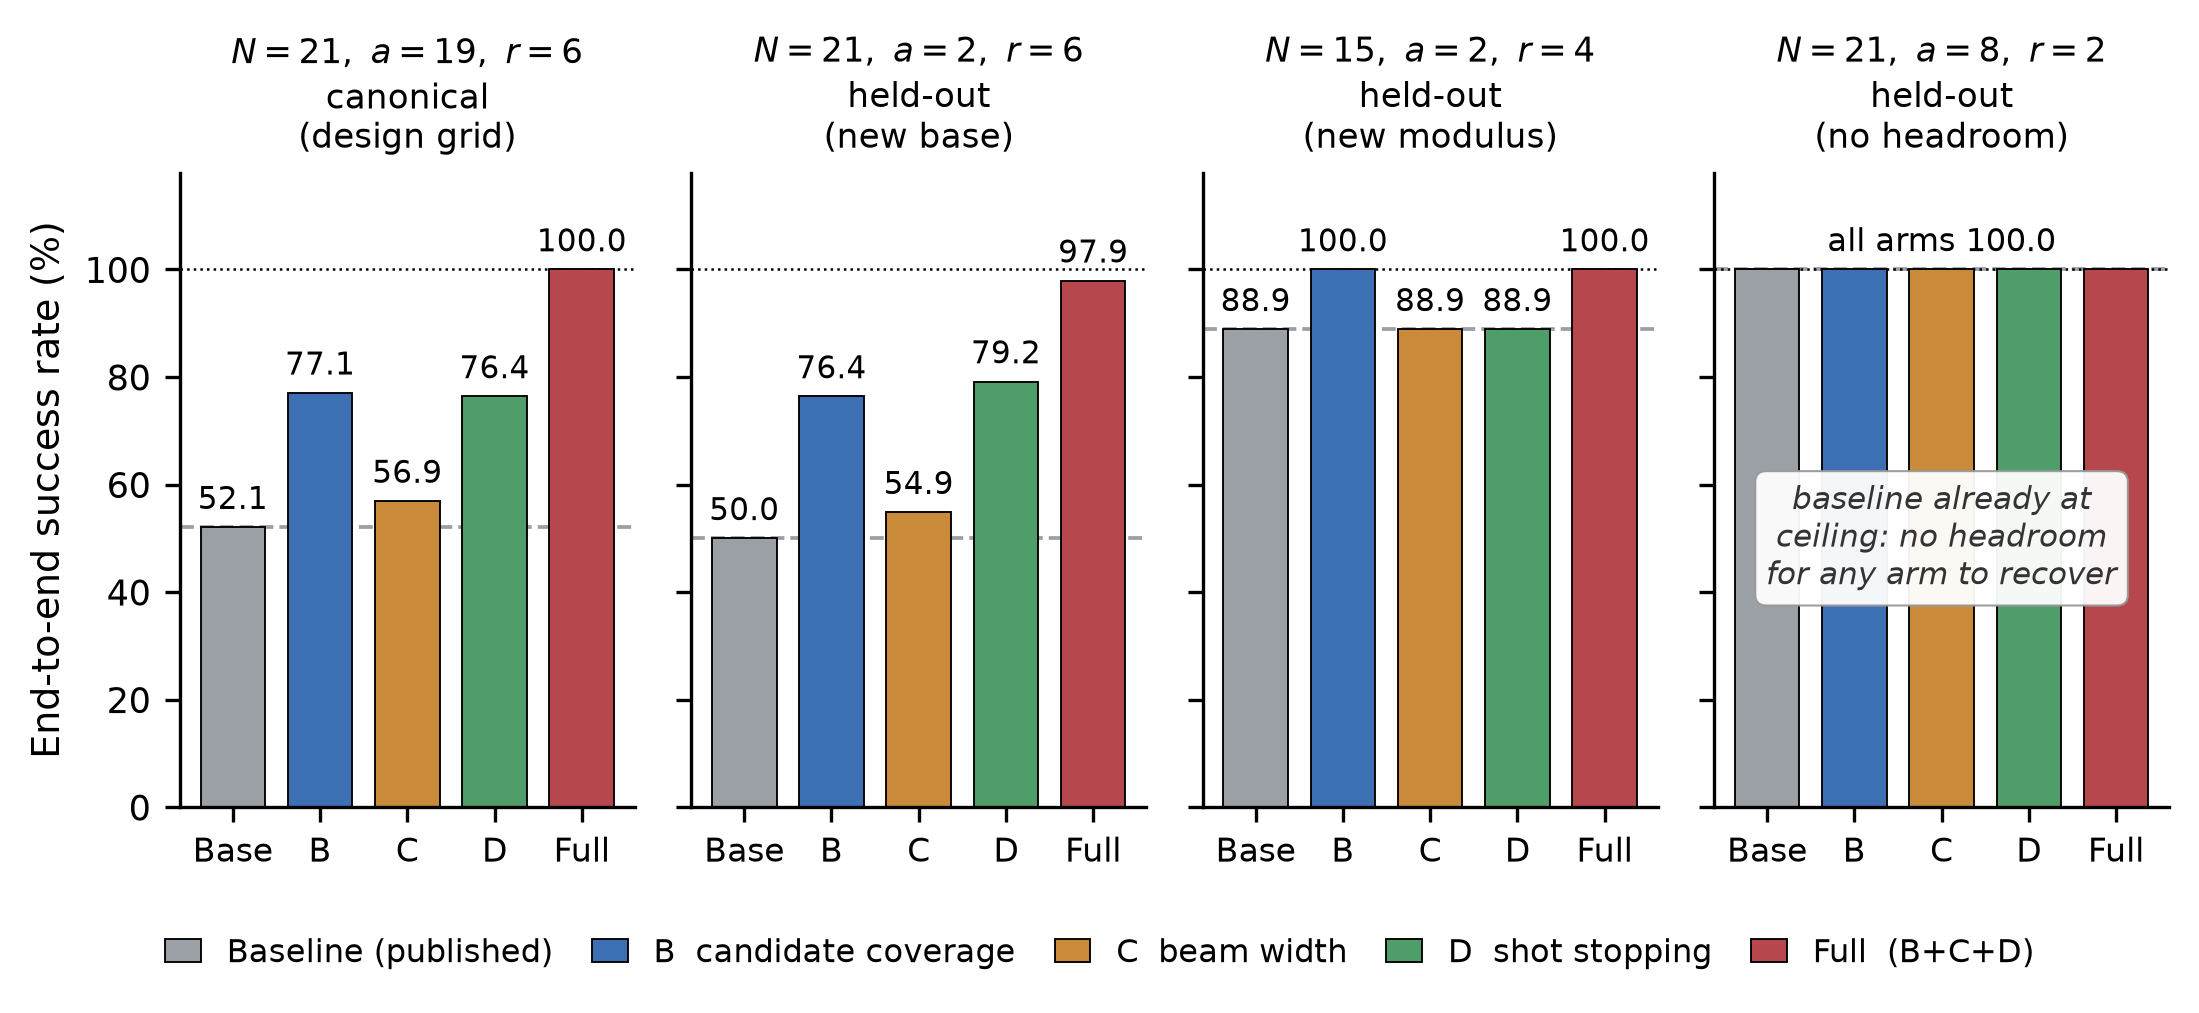
\includegraphics[width=0.94\linewidth]{../Data/failure_study/plots/paper_fig3_heldout.png}
\caption{\textbf{Does the canonical result survive on instances the
modules were never tuned against?} Per-arm end-to-end success on the
canonical instance (left) and the three pre-specified held-out
instances, 144 seed-paired trials each. Dashed line: that panel's
baseline. Dotted line: the 100\% ceiling. The canonical effect replicates
on $(N{=}21,a{=}2,r{=}6)$, a base never used in design, at 97.9\% rather
than 100\%. Headroom shrinks left to right: on $(N{=}15,a{=}2,r{=}4)$
only B and Full move the result, and on $(N{=}21,a{=}8,r{=}2)$ the
published pipeline already succeeds on every trial, so no arm can
demonstrate anything --- a ceiling effect, not a null effect. Module C
changes nothing on either right-hand instance. Rendered from
\texttt{phase6\_ablation\_diagnostics.csv} and
\texttt{phase7\_heldout\_*.csv}.}
\label{fig:heldout}
\end{figure}

\subsection{Matched-resource controls: what is the confidence statistic
actually buying?}
\label{sec:matched}

Every module works by spending more than baseline, which raises the
strongest objection available against this paper and one the ablation of
Sec.~\ref{sec:results} cannot answer: perhaps the gains have nothing to
do with confidence guidance, and any comparable budget increase ---
however allocated --- would do as well. Stage 3 tests exactly this, giving
the Baseline code path each adaptive arm's own realised budget spread
uniformly, with no confidence computation anywhere in the control
(Table~\ref{tab:matched}, Fig.~\ref{fig:matched}).

\textbf{No individual module is distinguishable from its matched
control.} Module B and its candidates-matched control both succeed on
77.1\% of trials, differing on two trials in opposite directions
($b{=}1$, $c{=}1$, $p=1.00$). Module C and its beam-matched control agree
on every single trial ($b{=}c{=}0$, $p=1.00$). Module D reaches 76.4\%
against its control's 73.6\% --- $+2.8$ pp with an interval spanning zero
($[-6.9,+11.8]$, $b{=}22$, $c{=}26$, $p=0.67$), 48 discordant trials
split almost evenly. None comes close to surviving Holm correction
(\SItables{}).

\textbf{The combination is distinguishable.} Full reaches 100\% against
the shots-matched control's 73.6\%: $+26.4$ pp (95\% CI $[+19.4,+33.3]$),
fixing 38 trials the control failed and breaking none ($b{=}0$, $c{=}38$,
$p=7.3\times10^{-12}$). This is the weaker of the two directions the
comparison could have been run in, since the control was matched on shots
alone while Full also widened candidates and beam --- a caveat we return
to below.

\paragraph{What this licenses us to claim, and what it does not.} It does
not license the claim that placing budget by confidence beats placing the
same budget uniformly: at the instance sizes we can reach it does not,
and we found no evidence that it does. What the controls establish is
narrower --- the statistic \emph{recovers} a budget as good as an
oracle-matched uniform one \emph{without being told what that budget
is}. The controls are not algorithms anyone could run: each is built from
diagnostics recorded while watching the adaptive rule make its choices on
that very trial. Sec.~\ref{sec:discussion} develops what this does and
does not support.

There is a second, quantitative reading. The budgets the controls were
handed are large --- a mean of $43.7$ extra shots per window on a grid
whose starved settings are 4--16, a matched candidate count of $4.29$
against a baseline $k\in\{1,2\}$, a matched beam width of $21.1$ against
$P\in\{1,2\}$ (\SItables{}) --- and the adaptive rules arrived at these
multiples from the counts alone. That the uniform version of the same
total performs equally well is a statement about \emph{this} regime: few
windows, small orders, and ambiguity spread fairly evenly across windows.
We would expect the two to separate where ambiguity is concentrated in a
minority of windows, but we have no instance in reach that exhibits that
concentration, so we do not claim it.

\paragraph{How exact is the matching?} The beam-matched control is
exact: $P'$ is already a trial-level scalar, and the control receives
that trial's value unchanged, so its realised beam width equals module
C's on every trial. The other two approximate a non-uniform per-window
allocation by its mean, and the direction of the residual error matters,
so we report it. The candidates-matched control received a mean
$k=4.29$ against module B's mean realised $m_w=4.25$: it was, if
anything, \emph{over}-matched, which makes B's null result harder rather
than easier to obtain. The shots-matched control received a mean of
$43.70$ extra shots per window against the $43.82$ module D actually
drew --- under-matched by $0.3\%$, a shortfall far too small to account
for D's $+2.8$~pp point estimate, and in the direction that favours D.
Neither residual changes the conclusion.

\paragraph{The remaining limit of the controls.} Matching a non-uniform
allocation by its mean is the natural uniform counterpart, but it is not
the only possible one, and a differently-constructed control could
behave differently. More importantly, \textbf{no control matches all
three budgets simultaneously against the Full arm}. The
Full-vs-control comparison equalises shots only, so its $+26.4$~pp
cannot be attributed to confidence guidance alone --- part of it is
simply the candidate and beam budget that the control never received.
Constructing a fully matched three-way control is a direct extension of
the released instrumentation and is the single experiment we would add
next; we flag its absence rather than let the $p=7.3\times10^{-12}$
stand unqualified.

\begin{table}[htbp]
\centering\small
\caption{Matched-resource controls on the canonical 144-trial grid. Each
control runs the Baseline code path, with all module flags disabled, at
the uniform budget derived from that trial's own adaptive diagnostics.
$b$ = trials where the control succeeded and the adaptive arm failed;
$c$ = the reverse. The upper block is the reference gain over an
unmodified baseline; the lower block is the comparison that matters.}
\label{tab:matched}
\resizebox{\linewidth}{!}{%
\begin{tabular}{@{}lccccc@{}}
\toprule
Comparison & Reference & Arm & Diff.\ [95\% CI] & $(b,c)$ & Exact $p$ \\
\midrule
\multicolumn{6}{@{}l}{\emph{Controls do improve on an unmodified baseline}}\\
candidates-matched vs.\ Baseline & 52.1\% & 77.1\% & $+25.0$ pp $[+18.1,+33.3]$ & $(2,38)$ & $1.5\times10^{-9}$ \\
beam-matched vs.\ Baseline       & 52.1\% & 56.9\% & $\phantom{0}+4.9$ pp $[+1.4,+8.3]$ & $(0,7)$ & $1.6\times10^{-2}$ \\
shots-matched vs.\ Baseline      & 52.1\% & 73.6\% & $+21.5$ pp $[+11.8,+31.3]$ & $(13,44)$ & $4.7\times10^{-5}$ \\
\midrule
\multicolumn{6}{@{}l}{\emph{Adaptive arm vs.\ its own matched control}}\\
B vs.\ candidates-matched & 77.1\% & 77.1\% & $\phantom{0}+0.0$ pp $[-2.1,+2.1]$ & $(1,1)$ & $1.00$ \\
C vs.\ beam-matched       & 56.9\% & 56.9\% & $\phantom{0}+0.0$ pp $[+0.0,+0.0]$ & $(0,0)$ & $1.00$ \\
D vs.\ shots-matched      & 73.6\% & 76.4\% & $\phantom{0}+2.8$ pp $[-6.9,+11.8]$ & $(22,26)$ & $0.67$ \\
\textbf{Full vs.\ shots-matched} & \textbf{73.6\%} & \textbf{100.0\%} & $\mathbf{+26.4}$ \textbf{pp} $[+19.4,+33.3]$ & $(0,38)$ & $7.3\times10^{-12}$ \\
\bottomrule
\end{tabular}
}
\end{table}

\begin{figure}[htbp]
\centering
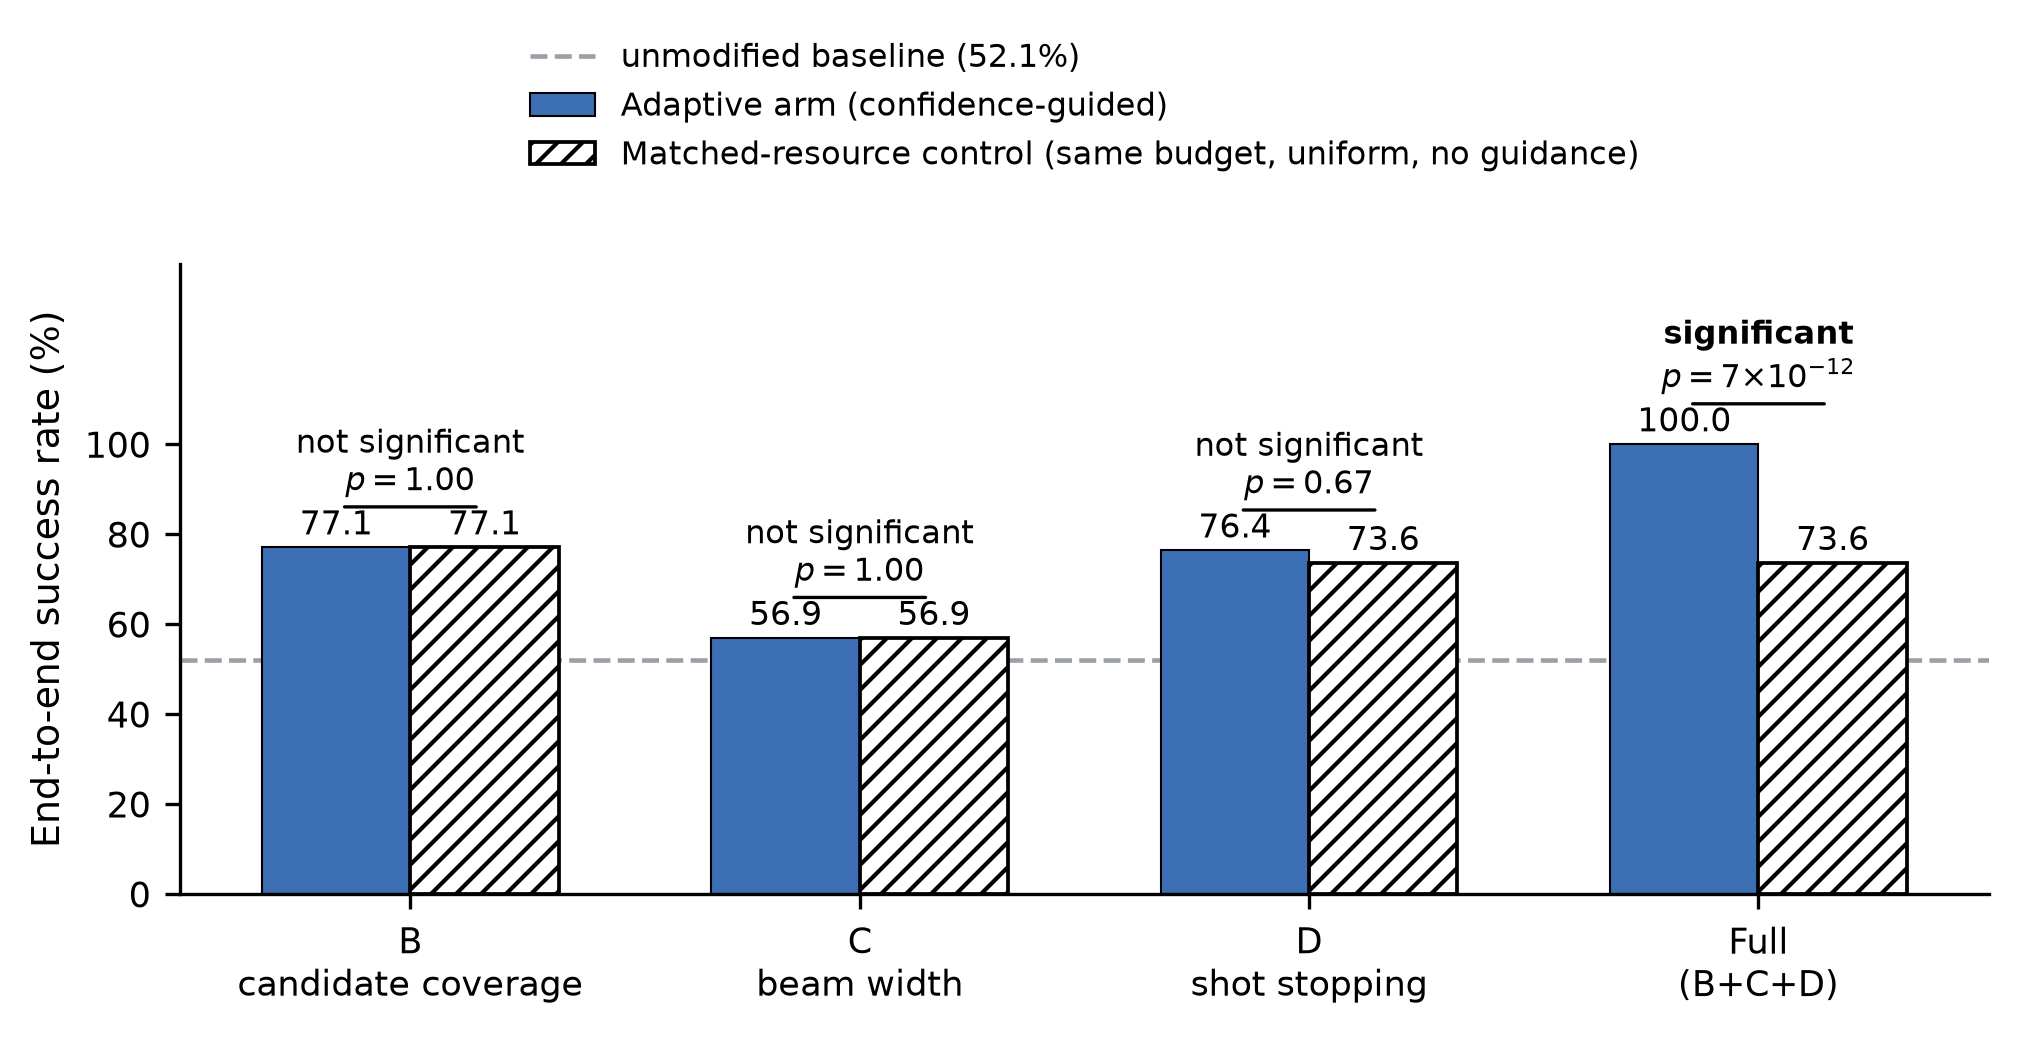
\includegraphics[width=0.94\linewidth]{../Data/failure_study/plots/paper_fig4_matched_resource.png}
\caption{\textbf{Is the gain due to confidence guidance, or to the size
of the budget it requests?} Each adaptive arm beside a control run
through the baseline code path at that arm's \emph{own} realised budget,
spread uniformly, with no confidence computation anywhere. Canonical
grid, 144 seed-paired trials. \textbf{The central result is the three
``not significant'' labels}: taken one at a time, none of the modules
outperforms an equally-resourced uniform allocation. Only the full
combination separates from its control, and that control is matched on
shots alone (Limitation~2). The controls are oracles,
not competitors --- their budgets could only be known after watching the
adaptive rule choose them. Rendered from
\texttt{phase7\_matched\_resource.csv}.}
\label{fig:matched}
\end{figure}

\subsection{Calibration analysis: $\Cw$ provides useful ranking
information but is not a calibrated probability estimate}
\label{sec:calibration}

Module D thresholds on $\Cw$, so it matters whether $\Cw$ means what its
scale suggests. We tested this on 2{,}687 per-window observations from
579 recaptured trials, pairing each window's predicted $\Cw$ against
ground truth: whether the observed top-1 pattern's \emph{true} noiseless
marginal really does exceed the top-2 pattern's, computed per window
specification by exact statevector simulation rather than by sampling
(\SIcalib{}).

\textbf{$\Cw$ is systematically overconfident.} The raw Brier score
\cite{brier1950} is $0.2239$, only marginally better than the $0.25$ a
constant always-0.5 forecast would achieve. In the top predicted decile
($\Cw\in(0.9,1.0]$, mean prediction $0.96$) the observed correctness rate
is $0.79$. Windows that satisfy module D's stopping rule at
$\varepsilon=0.05$ are therefore wrong roughly 21\% of the time, not 5\%.
Figure~\ref{fig:calib} shows the reliability diagrams.

This is the predicted cost of assumption (A2) being false: $b^{(1)}_w$
and $b^{(2)}_w$'s counts are negatively correlated marginals of one
Dirichlet posterior, not independent Binomials, and ignoring that
correlation pushes $\Cw$ toward more extreme values than a joint
comparison would. Isotonic regression \cite{zadrozny2002} recalibrates
the raw score to a Brier of $0.1988$ --- but that is an \emph{in-sample}
fit on the same 2{,}687 observations, with no held-out split, so it bounds
what recalibration could achieve rather than estimating out-of-sample
calibration. What it does establish is that the miscalibration has
correctable structure --- a monotone distortion, not noise --- which is
the property that makes the raw statistic usable as a ranking signal at
all. Bin-level data are in \SIcalib{}.

\textbf{We deliberately do not ship the recalibration in the default
decision rule}, and we want to be precise about why. The isotonic model
is fitted on this corpus; wiring it into module D would make the
shipped stopping rule depend on a fit whose generalisation to other
instances, orders, and window geometries we have not tested, and would
break the correspondence between the shipped configuration and the
ablation reported in Sec.~\ref{sec:results}, which thresholds on raw
$\Cw$. The consequence must be stated without softening:
\textbf{$\varepsilon$ is a tuning parameter for a heuristic stopping
rule, not a statistically guaranteed error tolerance, despite its name.}

None of this contradicts module D's measured effect: a miscalibrated but
monotone statistic (Table~\ref{tab:properties}) can be a serviceable
\emph{relative} signal for ``resample this window before that one'' while
being a poor \emph{absolute} probability, and only the ordering is
load-bearing in Sec.~\ref{sec:moduleD}. Two consequences follow for an
adopter: $\varepsilon$ must be tuned empirically rather than set from a
desired error rate, and any extension consuming $\Cw$ \emph{as} a
probability --- combining it across windows, or propagating it into a
downstream posterior --- would be unsound without out-of-sample validated
recalibration, which we have not performed.

\begin{figure}[htbp]
\centering
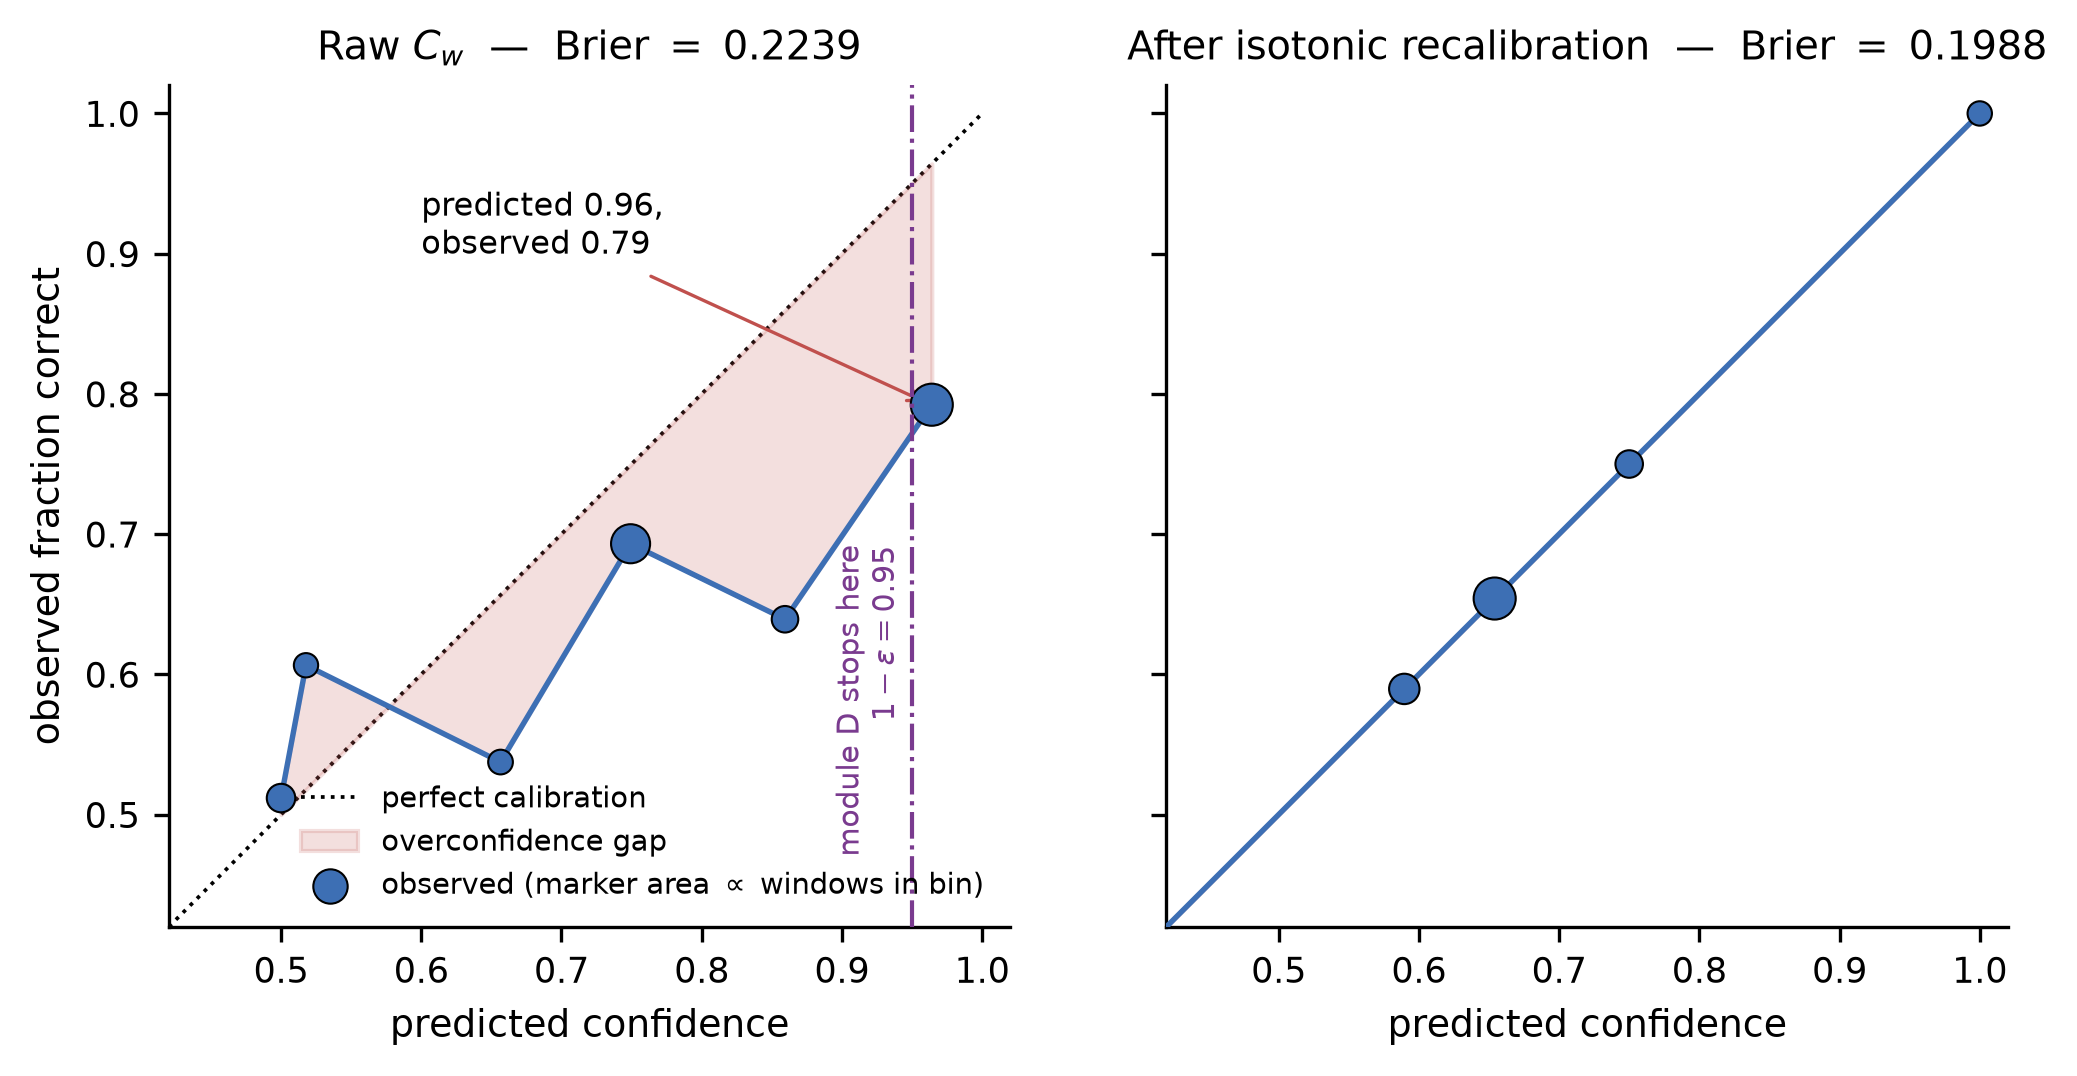
\includegraphics[width=0.94\linewidth]{../Data/failure_study/plots/paper_fig5_calibration.png}
\caption{\textbf{Does $\Cw$'s numerical value behave like a
probability?} Reliability of $\Cw$ over 2{,}687 per-window observations
from 579 trials; marker area is proportional to the number of windows in
the bin. \emph{Left:} raw $\Cw$ lies below the diagonal across the upper
range --- the shaded region is the overconfidence gap --- with Brier
$0.2239$ against $0.2500$ for a constant $0.5$ forecast. The dash-dotted
line marks module D's stopping threshold $1-\varepsilon=0.95$: windows
that halt there sit in a bin whose mean prediction is $0.96$ but whose
observed correctness is $0.79$. \emph{Right:} isotonic recalibration
reduces the Brier score to $0.1988$. \textbf{The right-hand panel is an
in-sample fit} --- isotonic regression places the bins on the diagonal by
construction --- so it establishes that the miscalibration is
\emph{correctable in principle}, not that a recalibrated $\Cw$ would
generalise. It is a diagnostic artifact and is deliberately not used by
the shipped stopping rule. Rendered from
\texttt{phase6\_calibration.csv}.}
\label{fig:calib}
\end{figure}

\subsection{Baseline reproduction as a validity check}
\label{sec:baselinecheck}

Invariant~\ref{prop:baseline} asserts that the framework with all modules
disabled \emph{is} the published pipeline. That is a claim about code
structure, so measurement cannot establish it --- but measurement can
falsify it, and we checked two ways.

The Baseline arm's success rate reproduces the original combined-stress
figure across three measurements: 52.1\% in the original failure-mode
campaign, 52.1\% in the ablation reported here, and 51.1\% in an interim
run at 139 of 144 trials.\footnote{The interim analysis predates the five
heaviest configurations finishing. The full 144-trial results reported
throughout supersede it; conclusions are unchanged.} The first is not a
re-run of the same function: the original campaign drove the published
pipeline through its own entry point, whereas the Baseline arm is the
adaptive entry point with all flags disabled. Their agreement is
therefore evidence \emph{across} implementations, which a single-function
re-run could not provide.

The second check is stronger than agreement between rates. The
instrumented re-run of Sec.~\ref{sec:design} was gated on reproducing the
recorded per-trial outcomes of \emph{every} arm exactly --- trial by
trial, not in aggregate --- and did so on all 144 trials in all five arms.
Adding the instrumentation that Sec.~\ref{sec:matched} depends on
therefore changed no result, and the seed-paired determinism the whole
design rests on holds in practice rather than merely in principle. Had it
not, the matched-resource controls would have been uninterpretable, since
each is built from a diagnostic recorded during that run.

\subsection{Discussion}
\label{sec:discussion}

\textbf{The central result of this study is not that confidence-guided
allocation has been shown to outperform an equal uniform allocation of
the same total resources.} The matched-resource controls do not support
that claim. What the evidence shows is that the proposed rules can infer
and deploy a workable reconstruction budget from the observed measurement
data, whereas the original pipeline requires that budget to be selected
manually in advance. Every statement elsewhere in this article is scoped
to that reading.

Three findings sit uneasily together at first reading: the combination
of all three modules removes essentially every failure in the regime
where failures occur; individually, no module beats a budget-matched
control; and those controls are themselves not implementable, since they
require knowing in advance what the adaptive rule would have chosen. The
reconciliation is that the modules are not competing with a well-chosen
fixed budget --- they are competing with the problem of choosing one.
Sec.~\ref{sec:motivation} showed that no single starved budget causes
failure while three starved together cause it half the time, so a
practitioner cannot diagnose which knob to turn from a failure alone, and
the correct setting varies cell by cell. That the rule's allocation
performs like an oracle-matched uniform one is the strongest available
evidence that it picks sensible values.

Table~\ref{tab:adopt} states what we would recommend a practitioner
adopt, and on what evidence. The modules are \emph{not} equally
supported, and presenting them as a uniform package would misrepresent
the study.

\begin{table}[htbp]
\centering\small
\caption{Adoption guidance. ``Evidence'' summarises
Secs.~\ref{sec:results}--\ref{sec:matched}; costs are from
Sec.~\ref{sec:cost}.}
\label{tab:adopt}
\begin{tabular}{@{}lp{0.36\linewidth}p{0.36\linewidth}@{}}
\toprule
Module & Evidence & Recommendation \\
\midrule
\textbf{B} coverage
 & Largest and most stable effect; improved every instance with
   headroom; broke at most two trials anywhere.
 & \textbf{Adopt first.} Cheapest of the three: no additional circuit
   execution, same asymptotic class as the code it replaces. \\[3pt]
\textbf{D} shot stopping
 & Large where shots bind, nil where they do not; the most two-sided
   per-trial behaviour in the study.
 & Adopt where sampling is cheap relative to a failed run; it dominates
   wall-clock cost whenever it fires. \\[3pt]
\textbf{C} beam width
 & Fails Holm correction; null on two of three held-out instances;
   indistinguishable from its matched control on every trial.
 & \textbf{Do not enable alone.} Retained in the Full configuration only
   because it provably never narrows the beam and 20 attributed failures
   needed both budget axes relaxed together. \\
\bottomrule
\end{tabular}
\end{table}

None of this is in tension with the calibration result of
Sec.~\ref{sec:calibration}: module D's stopping rule needs $\Cw$ to order
windows correctly, not to state a correct probability. Where the
miscalibration does cost something is the choice of $\varepsilon$, which
consequently has no principled setting and was left at its default.

% =====================================================================
\section{Limitations}
\label{sec:limitations}

We group these into six, ordered by how much each constrains what a
reader may conclude. Each names what would close it; several cannot be
closed by writing.

\paragraph{1. External validity and evaluation scope.}
Every result is at $N\in\{15,21\}$ with $r\in\{2,4,6\}$, noiseless, and
in simulation. \emph{The instance ceiling is not a choice}: the
modular-arithmetic layer of our reference implementation is a dense
unitary whose compilation time rises from $0.4$\,s at 5 work qubits to
$42$\,s at 7 and exceeds a $45$\,s timeout at 8 ($N\approx143$),
foreclosing larger instances before a shot is sampled; within that
ceiling only $N\in\{15,21\}$ admits an odd two-prime modulus with the
even, non-trivial order factor extraction requires. At these orders the
continued-fraction search is very forgiving, and that forgiveness
confounds \emph{any} claim about classical-stage robustness --- the $r=2$
instance, where the unmodified baseline already succeeds on every trial,
demonstrates it directly. \emph{The noiseless scope is a choice}, made to
isolate the mechanism under test, and it leaves the 27\% of
characterisation-campaign failures attributed to noise outside the
evaluated regime. Modules B and C act only on already-sampled counts, but
module D is more exposed: under a noise floor, additional shots can
sharpen confidence in a wrong pattern while consuming the $\Smax$ budget.
We make no claim about behaviour under noise in either direction.
Simulation-only status further excludes the queueing, calibration-drift
and per-shot cost structures D would meet on hardware. \emph{Closing
these:} a reversible modular-arithmetic circuit \cite{cuccaro2004} for
the ceiling; re-running the existing five-arm grid with the noise models
already in the released code, which needs compute rather than new
method.

\paragraph{2. Attribution of the gain to allocation rather than budget.}
Against matched-resource controls, no individual module is
distinguishable from a control given the same realised budget spread
uniformly (Sec.~\ref{sec:matched}). We therefore do not claim that
per-window placement is intrinsically better; the supported claim is that
the rule recovers an oracle-quality budget without being given one. Three
residual gaps qualify even that. \textbf{No control matches all three
budgets against the Full arm}: the Full-vs-control comparison equalises
shots only, so part of its $+26.4$~pp is candidate and beam budget the
control never received, and the figure cannot be attributed to confidence
guidance alone. The shots- and candidates-matched controls approximate a
non-uniform allocation by its mean; only the beam-matched control is
exact (residuals and their directions are quantified in \SItables{}). And
we have no instance whose ambiguity is concentrated in a minority of
windows --- the regime where we would predict placement to separate from
uniform allocation. \emph{Closing these:} a three-way matched control, a
direct extension of the released instrumentation and the single
experiment we would add next.

\paragraph{3. The confidence model.}
$\Cw$'s independence assumption (A2) is measurably false, and the
calibration study quantifies the cost: raw Brier $0.2239$ against
$0.2500$ for a constant $0.5$ forecast, with the top predicted bin at
$0.96$ predicted against $0.79$ observed. The consequence is that
$\varepsilon$ names an error target but delivers a heuristic threshold on
an uncalibrated statistic; it must be tuned empirically rather than set
from a desired error rate, and any extension consuming $\Cw$ as a
probability would be unsound. The isotonic recalibration is deliberately
not wired into the shipped rule, so that the shipped configuration is the
one that was ablated --- and in any case it was fitted and evaluated
in-sample on the same 2{,}687 observations, so its $0.1988$ bounds what
recalibration could achieve rather than estimating out-of-sample
performance. Separately, $\Cw$ compares only the top two patterns (A3),
so a genuine three-way near-tie is not flagged as low-confidence: a
structural blind spot rather than a tuned trade-off, accepted given
$\ell_w\le6$ throughout our corpus. \emph{Closing these:} a
Dirichlet-joint formulation of Eq.~\eqref{eq:cw}; a held-out calibration
split.

\paragraph{4. Module-specific evidence.}
\textbf{Module C is not supported as an independent intervention.} It
fails Holm correction at the confirmatory family size
(\SItables{}), is null on two of three held-out instances, and
agrees with its matched control on every trial. Its rule is also
heuristic: $\mathrm{expanded}$ counts ambiguous windows and is not a
derived sufficient beam width. We recommend against enabling it alone and
retain it in the Full configuration only on the strength of its proven
inability to narrow the beam and the 20 compounded failures that needed
both budget axes relaxed together. \textbf{Module B carries no population
coverage guarantee}: $\dcov$ bounds coverage of the observed sample, not
the probability that the true pattern is retained
(Table~\ref{tab:properties}); closing that requires a finite-sample
concentration bound we neither derive nor implement. \textbf{Per-trial
regressions are real}: enabled alone, B turned two canonical-grid
successes into failures and D six, and on $(N{=}15,a{=}2)$ D broke
exactly as many trials as it fixed. The Full arm regressed no trial on
any instance, but a practitioner enabling a single module should expect a
small rate of reversals.

\paragraph{5. Parameters and statistical scope.}
$\varepsilon$ and $\dcov$ were used at their defaults
(Sec.~\ref{sec:parameters}) because those defaults already produced large
effects, so no calibration failure prompted a search; we do not know how
sensitive the reported effects are to them, and a looser $\varepsilon$
might capture most of D's benefit at lower sampling cost. The canonical
grid also served both to identify budget starvation and to evaluate the
fix --- the held-out instances of Sec.~\ref{sec:heldout} address that
circularity, but they broaden \emph{which} instance is tested rather than
supplying a harder one. And McNemar's test speaks to one evaluation set:
two repeats per grid cell do not characterise run-to-run variability.

\paragraph{6. Deliberate scope exclusions.}
Window geometry is fixed at configuration time and never revised in
response to confidence (A5), so a separate and sharply-defined failure
mode --- within ${\sim}1\%$ of a window's $0.5$ ambiguity boundary the
winning bucket is unstable across repeated identical measurements --- is
untouched by this framework, which by construction cannot revise geometry
without regenerating circuits. Each window is also allocated
independently, with no shared budget across windows (A4); we did not
analyse jointly constrained allocation because no experiment in our
harness imposes such a budget, which is itself a gap in the evaluation
rather than evidence that coupling would not help.

% =====================================================================
\section*{Ethics statements}
This work involved no human participants, no animal subjects, and no data
collected from social media platforms. All data are generated by
numerical simulation.

\section*{CRediT author statement}
\noindent
Sanjay Lakshmanan R: Conceptualization, Methodology, Software,
Validation, Formal analysis, Investigation, Data curation,
Writing -- original draft, Writing -- review \& editing, Visualization.

\section*{Declaration of competing interest}
The author declares no known competing financial interests or personal
relationships that could have appeared to influence the work reported in
this paper.

\section*{Reproducibility}

Every numeric claim in this article is a mechanical summary of a released
result file; \SIartifacts{} maps each file to the script
that produced it and the section that consumes it. Three properties make
the results reproducible rather than merely re-runnable.

\textbf{Trials are deterministic given their seed.} Each trial's seed is
derived from its grid coordinates and seeds Aer's sampling, so re-running
any cell reproduces its counts exactly. This is what licenses the
five-arm within-subjects comparison, and it was verified rather than
assumed: the instrumented re-run of Sec.~\ref{sec:design} reproduced all
144 canonical trials, in all five arms, bit-for-bit.

\textbf{The analysis is fully specified}: exact two-sided binomial
McNemar; percentile bootstrap with $B=2000$ resamples at fixed seed 0
over paired per-trial differences; Holm correction over the family of
nine declared in Sec.~\ref{sec:stats}.

\textbf{Long runs are resumable.} A completed trial is skipped on restart
by its seed, so an interrupted campaign resumes without altering any
result --- necessary in practice, as the heaviest cells take tens of
minutes each.

One caveat for anyone recomputing our tables from the released
\emph{summary} CSVs: their two discordant-count columns,
\texttt{baseline\_only\_fixed\_count} and \texttt{arm\_only\_broke\_count},
hold the reverse of what their names suggest --- the first is $b$
(baseline succeeded, arm failed), the second $c$. The per-trial CSVs are
unambiguous and are what every table here was built from.

\section*{Code availability}
The complete implementation --- quantum circuits, classical
reconstruction, the adaptive modules, and every experiment script named
in \SIartifacts{} --- is released under the Apache-2.0 licence at
\url{https://github.com/Shadow-46/QuantumPhaseReconstruction}. An archived snapshot will be deposited in
a persistent repository and its DOI supplied at acceptance. The modules
described in this article are implemented in
\texttt{Reconstruction/\allowbreak{}confidence.py} (the statistic $\Cw$),
\texttt{Reconstruction/\allowbreak{}candidate\_\allowbreak{}generation.py} (module B),
and the adaptive entry point in \texttt{Experiments/\allowbreak{}harness.py}
(modules C and D, and the switchable reconstruction path of
Invariant~\ref{prop:baseline}). Each executable module carries a self-test
that runs without arguments.

\section*{Data availability}
All raw per-trial records, per-window recaptured counts, summary tables,
and figures are released with the code at the same location. No data were
obtained from third parties, and no dataset is under embargo.

\section*{Supplementary material}
A Supplementary Information document accompanies this article, containing
the complete derivations, the full audit record, the extended statistical
and resource tables, the bin-level calibration data, and the artifact
map. It is not required to understand the method or to judge the central
claims; it is what allows them to be verified independently. The released
data additionally contain the per-cell outcome grids for all five arms on
all four instances ($4\times144$ trials with realised $m_w$, $P'$ and
$S_w$ diagnostics), the 2{,}687-row per-window calibration record, the
full sweeps of the preceding failure-mode campaign, and the plotting
scripts that render every figure.

% =====================================================================
\bibliographystyle{elsarticle-num}
\bibliography{refs}

\end{document}
